\documentclass[12pt]{ucsddissertation}
% mathptmx is a Times Roman look-alike (don't use the times package)
% It isn't clear if Times is required. The OGS manual lists several
% "standard fonts" but never says they need to be used.
%\usepackage{mathptmx}

\usepackage{fontspec}
\usepackage{gfsdidot}          % makes math stuff look neat, but also overrides text stuff
\setmainfont{TeX Gyre Pagella} % forces back text stuff to look neat too
\setmonofont{DejaVuSansMono}   % monospace stuff should look neat too
%\renewcommand{\familydefault}{\sfdefault}
%\usepackage[scaled=1]{helvet}

\usepackage[NoDate]{currvita}
\usepackage{array}
%\usepackage{tabularx}
\usepackage{booktabs}
\usepackage{ragged2e}
\usepackage{microtype}

\usepackage[numbers]{natbib}
%\usepackage[style=ieee,natbib=true]{biblatex}

\usepackage{graphicx}

% Removed for preliminary appointment
% \usepackage{showframe}

% Valentin
\usepackage[dvipsnames]{xcolor} % must be loaded prior to tikz, pgfplots, etc.
\let\iint\relax
\let\iiint\relax
\let\iiiint\relax
\let\idotsint\relax
\usepackage{amsmath} % loaded by mathtools?
\usepackage{amssymb}
\usepackage[english]{babel}
\usepackage{calc}
\usepackage{caption}
\usepackage{color}
\usepackage{DejaVuSansMono}
\usepackage{dsfont}
\let\textlozenge\relax
\usepackage[inline]{enumitem}
\usepackage{environ}
\usepackage{etoolbox}
\usepackage{fontawesome}
\usepackage{forest}
\usepackage{graphicx}
\usepackage{longtable}
\usepackage{ltablex} \keepXColumns % Made me sad for appendix tables, where was it used?
\usepackage{makecell}
\usepackage{mathpartir}
%\usepackage{mathtools} % \coloneqq
\usepackage{mdframed}
\usepackage{minted}
\usepackage{multicol}
\usepackage[parfill]{parskip}
\usepackage{pgfplots}
\usepackage{pifont} % \ding
\usepackage{soul}
\usepackage{syntax}
\usepackage{tabularx}
\usepackage[skins,theorems]{tcolorbox}
\usepackage{tikz}
\usepackage{tikzpeople}
\usepackage{tikz-qtree}
\usepackage{xpatch}
\usepackage[breaklinks=true,pdfborder={0 0 0}]{hyperref}

% gfsdidot makes ∀ and ∃ super ugly, this reverts them to something fine
\DeclareSymbolFont{CMsymbols}{OMS}{cmsy}{b}{n}
\SetSymbolFont{CMsymbols}{bold}{OMS}{cmsy}{ub}{n}
\DeclareMathSymbol{\forall}{\mathord}{CMsymbols}{"38}
\DeclareMathSymbol{\exists}{\mathord}{CMsymbols}{"39}

\definecolor{color01}{HTML}{E6194B}
\definecolor{color02}{HTML}{3CB44B}
\definecolor{color03}{HTML}{FFE119}
\definecolor{color04}{HTML}{4363D8}
\definecolor{color05}{HTML}{F58231}
\definecolor{color06}{HTML}{911EB4}
\definecolor{color07}{HTML}{46F0F0}
\definecolor{color08}{HTML}{F032E6}
\definecolor{color09}{HTML}{BCF60C}
\definecolor{color10}{HTML}{FABEBE}
\definecolor{color11}{HTML}{008080}
\definecolor{color12}{HTML}{E6BEFF}
\definecolor{color13}{HTML}{9A6324}
\definecolor{color14}{HTML}{FFFAC8}
\definecolor{color15}{HTML}{800000}
\definecolor{color16}{HTML}{AAFFC3}
\definecolor{color17}{HTML}{808000}
\definecolor{color18}{HTML}{FFD8B1}
\definecolor{color19}{HTML}{000075}
\definecolor{color20}{HTML}{808080}
\definecolor{color21}{HTML}{FFFFFF}
\definecolor{color22}{HTML}{000000}

\def\mathunderline#1#2{\color{#1}\underline{{\color{black}#2}}\color{black}}

\forestset{
  default preamble={
    for tree={
      align=center,
      draw=black,
      edge={
        ultra thick,
      },
      edge path={
        \noexpand\path[\forestoption{edge}]
        (!u.parent anchor)
        -- +(0,-10pt)
        -| (.child anchor)
        \forestoption{edge label};
      },
      font=\bfseries,
      % inner sep=10pt,
      l sep=30pt,
      % line width=2pt,
      minimum height=20pt,
      minimum width=30pt,
      parent anchor=south,
      rectangle,
      ultra thick,
    }
  }
}

\newcolumntype{Y}{>{\centering\arraybackslash}X}

% defines safecoqinline, a command like coqinline but works in tabular
% environments
\makeatletter
\def\safecoqinline#1{%
\ifx\@footnotetext\TX@trial@ftn
\detokenize{#1}%
\else
\coqinline{#1}%
\fi}
\makeatother

\captionsetup{
  justification=centering,
}

\usetikzlibrary{arrows, calc, fit, positioning, shapes, tikzmark}

\tikzset{
bicolor/.style 2 args={
  dashed,dash pattern=on 4pt off 4pt,#1,
  postaction={draw,dashed,dash pattern=on 4pt off 4pt,#2,dash phase=4pt}
  },
}

\tikzstyle{Matching}=[
black,
dashed,
line width=3pt,
]

\tikzstyle{RoundedDottedPath}=[
densely dotted,
color05,
line width=3pt,
rounded corners=10pt,
]

\tikzstyle{RoundedRectangle}=[
dashed,
draw,
line width=3pt,
rounded corners=10pt,
]

\tikzstyle{NodeLabel}=[
black,
circle,
draw,
fill=white,
font=\bfseries,
inner sep=1pt,
ultra thick,
]

\graphicspath{ {./images/} }

\AtBeginDocument{%
	\settowidth\cvlabelwidth{\cvlabelfont 0000--0000}%
}

% Fix a mdframed bug where skipbelow is ignored
\makeatletter
\xpatchcmd{\endmdframed}
  {\aftergroup\endmdf@trivlist\color@endgroup}
  {\endmdf@trivlist\color@endgroup\@doendpe}
  {}{}
\makeatother

\surroundwithmdframed[
backgroundcolor=white,
linecolor=white,
skipabove=1em,
skipbelow=-0.5em,
leftmargin=10pt,
innertopmargin=1pt,
innerbottommargin=0pt
]{minted}

\setminted{
  % DO NOT use bgcolor, use mdframed instead
  %bgcolor=white,
  linenos=true,
  style=xcode,
  breaklines=true,
  encoding=utf8,
  fontsize=\small,
  baselinestretch=1,
}

% need bgcolor for the display to be nice in rules
\newmintinline{coq}{bgcolor=white}

% This works for some styles but not all, instead I hijack the tokens directly
% in background.tex

% \AtBeginEnvironment{minted}{%
%   \renewcommand{\fcolorbox}[4][]{#4}}
% \def\dontdofcolorbox{\renewcommand\fcolorbox[4][]{##4}}

% These do not seem to work...
% \xpatchcmd{\coqinline}{\minted@fvset}{\minted@fvset\dontdofcolorbox}{}{}
% \xpatchcmd{\mintinline}{\minted@fvset}{\minted@fvset\dontdofcolorbox}{}{}

\makeatletter
% \AtBeginEnvironment{minted}{\dontdofcolorbox}
% \def\dontdofcolorbox{\renewcommand\fcolorbox[4][]{##4}}
% \xpatchcmd{\inputminted}{\minted@fvset}{\minted@fvset\dontdofcolorbox}{}{}
% \xpatchcmd{\mintinline}{\minted@fvset}{\minted@fvset\dontdofcolorbox}{}{}

% \expandafter\def\csname PYGmonokai@tok@err\endcsname{
%   \def\PYGmonokai@tc##1{\textcolor[rgb]{0.59,0.88,0.31}{##1}}
%   \def\PYGmonokai@bc##1{\setlength{\fboxsep}{0pt}\colorbox[rgb]{0.88,0.00,0.06}{\strut ##1}}
% }
\makeatother

\makeatletter
\pgfdeclareshape{document}{
\inheritsavedanchors[from=rectangle] % this is nearly a rectangle
\inheritanchorborder[from=rectangle]
\inheritanchor[from=rectangle]{center}
\inheritanchor[from=rectangle]{north}
\inheritanchor[from=rectangle]{south}
\inheritanchor[from=rectangle]{west}
\inheritanchor[from=rectangle]{east}
% ... and possibly more
\backgroundpath{% this is new
% store lower right in xa/ya and upper right in xb/yb
\southwest \pgf@xa=\pgf@x \pgf@ya=\pgf@y
\northeast \pgf@xb=\pgf@x \pgf@yb=\pgf@y
% compute corner of ‘‘flipped page’’
\pgf@xc=\pgf@xb \advance\pgf@xc by-10pt % this should be a parameter
\pgf@yc=\pgf@yb \advance\pgf@yc by-10pt
% construct main path
\pgfpathmoveto{\pgfpoint{\pgf@xa}{\pgf@ya}}
\pgfpathlineto{\pgfpoint{\pgf@xa}{\pgf@yb}}
\pgfpathlineto{\pgfpoint{\pgf@xc}{\pgf@yb}}
\pgfpathlineto{\pgfpoint{\pgf@xb}{\pgf@yc}}
\pgfpathlineto{\pgfpoint{\pgf@xb}{\pgf@ya}}
\pgfpathclose
% add little corner
\pgfpathmoveto{\pgfpoint{\pgf@xc}{\pgf@yb}}
\pgfpathlineto{\pgfpoint{\pgf@xc}{\pgf@yc}}
\pgfpathlineto{\pgfpoint{\pgf@xb}{\pgf@yc}}
\pgfpathlineto{\pgfpoint{\pgf@xc}{\pgf@yc}}
}
}
\makeatother

% OGS recommends increasing the margins slightly.
\increasemargins{.1in}

% These are just for testing/examples, delete them
%\usepackage{trace}
%\usepackage{showframe} % This package was just to see page margins
%\usepackage[english]{babel}
%\usepackage{blindtext}
\overfullrule5pt
% ---

% Required information
\title{Front-end tooling for building and maintaining functional programs}
\author{Valentin Robert}
\degree{Computer Science}{Doctor of Philosophy}
% Each member of the committee should be listed as Professor Foo Bar.
% If Professor is not the correct title for one, then titles should be
% omitted entirely.
\chair{Professor Sorin Lerner}
%\cochair{Professor Gamma Delta} % Optional
% Your committee members (other than the chairs) must be in alphabetical order
\committee{Professor William Griswold}
\committee{Professor James Hollan}
\committee{Professor Ranjit Jhala}
\committee{Professor Todd Millstein}
\degreeyear{2018}

%%%%% General-purpose text macros %%%%%
\newcommand{\define}[1]{\emph{#1}}

\newcommand{\Language}[1]{\emph{#1}}
\newcommand{\Gallina}{\Language{Gallina}}
\newcommand{\Ltac}{\Language{Ltac}}
\newcommand{\Vernacular}{\Language{Vernacular}}

\newcommand{\Chick}{\Language{Chick}}
\newcommand{\Coq}{\Language{Coq}}
\newcommand{\Haskell}{\Language{Haskell}}
\newcommand{\JavaScript}{\Language{JavaScript}}
\newcommand{\PeaCoq}{\Language{PeaCoq}}
\newcommand{\RxJS}{\Language{RxJS}}
\newcommand{\SerAPI}{\Language{SerAPI}}
\newcommand{\Snap}{\Language{Snap}}
\newcommand{\TypeScript}{\Language{TypeScript}}

\newcommand{\OperatorColor}{purple}
\newcommand{\Operator}[1]{\textcolor{\OperatorColor}{\ #1\ }}
\newcommand{\Entails}{\Operator{\vdash}}
\newcommand{\HasType}{\Operator{:}}

\newmintinline[mycoq]{coq}{fontsize=\small}
\newcommand{\coqinline}[1]{%
  \colorbox{monokaibg}{%
    \parbox[c][0.9em]{\widthof{\mycoq{#1}}}{\mycoq{#1}}%
  }%
}

\newcommand{\modified}[1]{\color{yellow}{#1}}
\newcommand{\repaired}[1]{\color{green}{#1}}

\newcommand{\rulename}[1]{$\LeftTirNameStyle{#1}$}

\newcommand{\RmApp}{Rm-App}
\newcommand{\RmPi}{Rm-Pi}
\newcommand{\InsApp}{Ins-App}

%%%%% Math-mode macros %%%%%

\newcommand{\opcolor}{purple}
\newcommand{\out}[1]{ \boxed{ \textcolor{teal}{#1} } }
\newcommand{\MathPatches}[3]{
  #1 % \overset{#2}{\mathbin{\textcolor{\opcolor}{\rightsquigarrow}}} \out{#3}
}

\newcommand{\App}{\$}
\newcommand{\Mod}{Mod}
\newcommand{\Drop}{Drop}
\newcommand{\Ins}{Ins}
\newcommand{\Keep}{Keep}
\newcommand{\Lam}{\lambda}

\newcommand{\oMod}{\overset{\mathtt{\Mod}}}
\newcommand{\oDrop}{\overset{\mathtt{\Drop}}}
\newcommand{\oIns}{\overset{\mathtt{\Ins}}}
\newcommand{\oKeep}{\overset{\mathtt{\Keep}}}

\newcommand{\Cons}{::}
\newcommand{\permute}[2]{ \overline{#2}^{\overset{#1}{\rightleftarrows} } }
\newcommand{\permuteOp}[2]{ \overset{\overset{#1}{\rightleftarrows}}{#2} }

\newcommand{\mkMathPiRaw}[4]{#3{\Pi} #4{#1} \rightarrow #2}
\newcommand{\mkMathPi}[5]{\mkMathPiRaw{(#2 : #1)}{#3}{#4}{#5}}


\newcommand{\MathCons}[2]{#1 \Cons #2}
\newcommand{\MathDrop}[1]{\oDrop{\Cons} #1}
\newcommand{\MathDropApp}[1]{\oDrop{\App} #1}
\newcommand{\MathDropLam}[1]{\oDrop{\Lam} #1}
\newcommand{\MathDropPi}[1]{\oDrop{\Pi} #1}
\newcommand{\MathHole}{\texttt{\_}}
\newcommand{\MathIns}[2]{#1 \oIns{\Cons} #2}
\newcommand{\MathInsApp}[2]{\mkMathApp{#1}{#2}{\oIns}}
\newcommand{\MathInsAppOp}{\oIns{\App}}
\newcommand{\MathInsLam}[2]{\mkMathLam{#1}{#2}{\oIns}{}}
\newcommand{\MathInsLamOp}{\oIns{\Lam}}
\newcommand{\MathInsPi}[3]{\mkMathPi {#1}{#2}{#3}{\oIns}{}}
\newcommand{\MathInsPiOp}{\oIns{\Pi}}
\newcommand{\MathLam}[2]{\mkMathLam{#1}{#2}{}{}}
\newcommand{\MathLams}[3]{\mkMathLam{#1}{#2}{}{\BarCount{#3}}}
\newcommand{\MathKeepPiOp}{\oKeep{\Pi}}
\newcommand{\MathMod}[2]{#1 \oMod{\Cons} #2}
\newcommand{\MathModAppOp}{\oMod{\App}}
\newcommand{\MathModLamOp}{\oMod{\Lam}}
\newcommand{\MathModPiOp}{\oMod{\Pi}}
\newcommand{\MathPermute}[2]{\permuteOp{#1}{\Cons} #2}
\newcommand{\MathPermuteLams}[2]{\permuteOp{#1}{\lambda} #2}
\newcommand{\MathPermutePis}[2]{\permuteOp{#1}{\Pi} #2}
\newcommand{\MathPi}[3]{\mkMathPi{#1}{#2}{#3}{}{}}
\newcommand{\MathPis}[4]{\mkMathPi{#1}{#2}{#3}{}{\BarCount{#4}}}
\newcommand{\MathReplace}[1]{#1} % \thickul{#1}}
\newcommand{\MathSame}{\mathds{1}}

\newcommand{\mkMathApp}[3]{#1 #3{ \$ } #2}

\newcommand{\RuleRProgSameNil}{
  {
    \inferrule*
    [lab=R-Prog-Same-Nil]
    {  }
    {\turnstile%
      { \denv{E}{\delta_E} }
      { \repairProg{[]}{\MathSame}{\MathSame} }
    }
  }
}

\newcommand{\RuleRProgModify}{
  {
    \inferrule*
    [lab=R-Prog-Modify]
    {
      {\turnstile%
        { \denv{E}{\delta_E} }
        { \repairVernac{v}{\delta_v}{\delta_v'} }
      }
      \and
      {\turnstile%
        { \denv{v \Cons{} E}{\MathMod{\delta_v'}{\delta_E}} }
        { \repairProg{p}{\delta_p}{\delta_p'} }
      }
    }
    {\turnstile%
      { \denv{E}{\delta_E} }
      { \repairProg{\MathCons{v}{p}}{\MathMod{\delta_v}{\delta_p}}{\MathMod{\delta_v'}{\delta_p'}} }
    }
  }
}


\setlength\parindent{0.5in}
%\titleformat\paragraph{\sectioningformatting\normalsize\bfseries}{\theparagraph}{1em}{}

% Start the document
\begin{document}
% Begin with frontmatter and so forth
\frontmatter
\maketitle
\makecopyright
\makesignature
% Optional
% \begin{dedication}
% \setsinglespacing
% \raggedright % It would be better to use \RaggedRight from ragged2e
% \parindent0pt\parskip\baselineskip
% In recognition of reading this manual before beginning to format the
% doctoral dissertation or master's thesis; for following the
% instructions written herein; for consulting with OGS Academic Affairs
% Advisers; and for not relying on other completed manuscripts, this
% manual is dedicated to all graduate students about to complete the
% doctoral dissertation or master's thesis.

% In recognition that this is my one chance to use whichever
% justification, spacing, writing style, text size, and/or textfont that
% I want to while still keeping my headings and margins consistent.
% \end{dedication}
% % Optional
% \begin{epigraph}
% \vskip0pt plus.5fil
% \setsinglespacing
% {\flushright
% True ease in writing comes from art, not chance,\\
% As those move easiest who have learn'd to dance.\\
% 'T is not enough to no harshness gives offence,---\\
% The sound must seem an echo to the sense.

% \vskip\baselineskip
% \textit{Alexander Pope}\par}
% \vfil
% \begin{center}
% You write with ease to show your breeding,\\
% But easy writing's curst hard reading.

% \vskip\baselineskip
% \textit{Richard Brinsley Sheridan}
% \end{center}
% \vfil
% \noindent Writing, at its best, is a lonely life. Organizations for
% writers palliate the writer's loneliness, but I doubt if they improve
% his writing. He grows in public stature as he sheds his loneliness and
% often his work deteriorates. For he does his work alone and if he is a
% good enough writer he must face eternity, or the lack of it, each day.

% \vskip\baselineskip
% \hskip0pt plus1fil\textit{Ernest Hemingway}\hskip0pt plus4fil\null

% \vfil
% \end{epigraph}

% Next comes the table of contents, list of figures, list of tables,
% etc. If you have code listings, you can use \listoflistings (or
% \lstlistoflistings) to have it be produced here as well. Same with
% \listofalgorithms.
\tableofcontents
\listoffigures
\listoftables

% Preface
% \begin{preface}
% \end{preface}

% Your fancy acks here. Keep in mind you need to ack each paper you
% use. See the examples here. In addition, each chapter ack needs to
% be repeated at the end of the relevant chapter.
\begin{acknowledgements}
I would like to thank Professor Sorin Lerner for his support as my advisor and
the chair of my committee.

Committing oneself to more than half a decade to a mentally-challenging,
ill-paying, self-motivated job seems like an awful idea.  Yet, it is the ordeal
that most graduate students choose, with little to no foresight as to where the
journey will lead them.  I would like to dedicate the next paragraphs to all
past, current, and future graduate students.

Throughout my six years as a graduate student, I have only been able to visit my
family for a total of three months, both my grandparents passed away after I was
unable to attend a Christmas with them, nor was I able to attend their
respective funeral.  I have needed to move twice, I have needed to TA seven
quarters, I have developed repetitive stress injuries in both my arms, and I
have loaned over \$10.000 to be able to bring this work to completion.

It was not without its worth though.

I have made a solid group of friends without which the journey would have been
too much to bear.  Zachary Tatlock brought me up to speed and offered me several
wonderful opportunities over the years.  Alexander Bakst was a great roommate,
and it was always great to go for a bike ride to go work the night at one of the
local coffee shops.  Neha Chachra was a great neighbour, and helped me work
through a lot of mental issues.  Marcela Mendoza also provided a lot of mental
support, personal growth, and both helped focus on working hard for several
years, and helped on rejuvenating from the worst grinds by being a great travel
companion.  Many recent new friends have made the final years of the journey
wonderful, with lots of music and enjoyable hangouts.  In particular, my partner
Andrea Frank provided a wonderful emotional support over the past year, and with
her roommate, John Renner, have provided the hosting without which I would not
have been financially able to complete my studies.

I would like to thank the rest of the UCSD Programming Systems group, who have
provided a great environment for research.  In particular, Eric Seidel has
always been tremendous at listening to my issues and offering the perfect,
appropriate technical pointers to resolve them.  My work would often have been
weeks behind without his help.

I would also like to thank the Gallium team of Inria, and in particular my
former mentor, Xavier Leroy, for his great mentorship and the confidence he
inspired in me.  Gabriel Scherer, Jonathan Protzenko, and Nicolas Pouillard,
among many others, have also been excellent lunch and coffee break companions,
who opened my eyes to many of the great concepts of the programming language
community.  Working with all of them was a daily delight.

Andrew Kennedy, who accepted me as an intern at Microsoft Research, gave me the
opportunity to work on a project where I got to improve my understanding of
\Coq{} at a tremendous speed, and introduced me to a project that I had not
believed possible.

I would like to thank the employees of Galois, Inc., where I gave a presentation
of my work earlier this year that was very well received, and followed by great
feedback.  In particular, David Christiansen pointed me to relevant literature
that made part of the work much easier.  It is an immense pleasure to have been
offered a position to work alongside the people I met that day.

Finally, I must thank my mother for her love and support.  This journey must
have been quite the ordeal for her too, and it was hard to convey the reasons
why I still had so much left to do before I was done.  Yet, she was
understanding, and always came through at the most difficult moments, no
questions asked.  Such care is commendable.

Chapter~\ref{peacoq}, in part, has been published in a series of blog
articles. The dissertation author was the primary investigator and author of
this material.

Chapter~\ref{chick}, in part, is currently being prepared for submission for
publication of the material.  The dissertation author was the primary
investigator and author of this material.

% I would like to acknowledge Professor Eta Theta for his support as the
% chair of my committee. Through multiple drafts and many long nights,
% his guidance has proved to be invaluable.

% I would also like to acknowledge the ``Smith Clan'' of lab~28, without
% whom my research would have no doubt taken fives times as long. It is
% their support that helped me in an immeasurable way.

% Chapter 2, in full, is a reprint of the material as it appears in
% Numerical Grid Generational in Computational Fluid Mechanics~2009.
% Smith, Laura; Smith, Jane~D., Pineridge Press,~2009. The dissertation
% author was the primary investigator and author of this paper.

% Chapter 3, in part, has been submitted for publication of the material
% as it may appear in Education Mechanics,~2009, Smith, Laura; Smith,
% Jane~D., Trailor Press,~2009. The dissertation author was the primary
% investigator and author of this paper.

% Chapter 5, in part is currently being prepared for submission for
% publication of the material. Smith, Laura; Smith, Jane~D\@. The
% dissertation author was the primary investigator and author of this
% material.

\end{acknowledgements}

% Stupid vita goes next
\begin{vita}
\noindent
\begin{cv}{}
\begin{cvlist}{}
\item[2012 - 2018] Doctorate of Philosophy, Computer Science, University of California San Diego
\item[2008 - 2012] Diploma of Engineering (Master's degree), ENSEIRB-MATMECA
\item[2006 - 2008] Classe pr\'eparatoire, Lyc\'ee Louis Barthou
\item[2001 - 2006] Baccalaur\'eat, Science specialization, Lyc\'ee Saint-Cricq
% \item[1996] Bachelor of Arts, University of California, Berkeley
% \item[1996--2000] U.S. Marines
% \item[2000--2002] Teaching Assistant, Department of Mechanical
% Engineering\\University of California, San Diego
% \item[2002--2006] Research Assistant, University of California, San
% Diego
% \item[2010] Doctor of Philosophy, University of California, San Diego
\end{cvlist}
\end{cv}

% This puts in the PUBLICATIONS header. Note that it appears inside
% the vita environment. It is optional.
\publications

\noindent Robert, V. and Leroy, X., 2012, December. A formally-verified alias
analysis. In International Conference on Certified Programs and Proofs
(pp. 11-26). Springer, Berlin, Heidelberg.

\noindent Ricketts, D., Robert, V., Jang, D., Tatlock, Z. and Lerner, S., 2014,
June. Automating formal proofs for reactive systems. In ACM SIGPLAN Notices
(Vol. 49, No. 6, pp. 452-462). ACM.

% This puts in the FIELDS OF STUDY. Also inside vita and also
% optional.
% \fieldsofstudy
% \noindent Major Field: Engineering (Specialization or Focused Studies)
% \vskip\baselineskip
% Studies in Applied Mathematics\par
% Professors Alpha Beta and Gamma Delta
% \vskip\baselineskip
% Studies in Mechanices\par
% Professors Epsilon Zeta and Eta Theta
% \vskip\baselineskip
% Studies in Electromagnetism\par
% Professors Iota Kappa and Lambda Mu
\end{vita}

% Put your maximum 350 word abstract here.
\begin{dissertationabstract}

Dependently-typed functional languages are increasingly popular, but due to the
complexity of their type systems, there is still a lot of friction in the user
experience, both for beginners who try to learn the concepts, and expert users
who must write and maintain complex code bases.  We explore ways to alleviate
those burdens by providing novel front-end tooling for this class of languages.

In order to help beginners, we explore new visualizations and automation
techniques, focusing on three pain points we identified in the learning process.
We evaluate, via a longitudinal user study and an A-B study, their effectiveness
in terms of learning to use those languages, enjoyment of the learning process,
and productivity on solving beginner-level exercises.

In order to help experts, we prototype a tool that helps in the refactoring of
programs, partially eliminating the tedium of propagating changes throughout
large code bases.  We evaluate this tool over a choice of refactoring
benchmarks, and show how it can be extended to support other languages than the
toy language we designed it for.  We evaluate one instance of this extension
technique to repair programs in the \OCaml{} language, a functional language
without dependent types, but with more features than our tool was built for.

% The Abstract begins here. The abstract is limited to 350 words for a
% doctoral dissertation. It should consist of a short statement of the
% problem, a brief explanation of the methods and procedures employed in
% generating the data, and a condensed summary of the findings of the
% study. The abstract may continue onto a second page if necessary. The
% text of the abstract must be double spaced.
\end{dissertationabstract}

% This is where the main body of your dissertation goes!
\mainmatter

% Optional Introduction
\begin{dissertationintroduction}

This thesis aims to design and evaluate novel tools for helping users of
functional programming languages and proof assistants.

Over the past couple decades, the concept of \emph{functional programming} has
flourished from an academic object of interest to a trending topic in both
academia and industry.  Concepts that used to be mostly relevant in the context
of functional programming languages, for instance, \emph{anonymous functions},
\emph{currying}, \emph{monads}, or \emph{dependent types}, are percolating into
many functional languages as well as mainstream imperative languages.

%%% Local Variables:
%%% mode: xetex
%%% TeX-master: "dissertation"
%%% End:


% This optional section is barely described in the OGS manual other than
% saying it is optional and that it appears in the table of contents
% between the Abstract and the first chapter.

% No formatting guidelines appear so presumably, it should be formatted
% like an ordinary chapter. It should appear after the
% \verb!\mainmatter! macro because it should start on page~1.
\end{dissertationintroduction}

% Too much
%\chapter{Background}\label{background}

This section provides a brief high-level introduction to basic concepts used in
the rest of the dissertation.

\section{Static typing}
\label{static-typing}

% Define static typing

% Discipline of prescribing valid programs from invalid ones

Programmers typically do not write programs by simply manipulating bits in the
computer's memory: most languages offer abstraction mechanisms that let their
users reason at a higher level.  One such high-level abstraction is the notion
of a \define{data type}.  A programmer will want to manipulate structured data
such as numbers, Boolean values, or compound values made out of different values
organized together in some fashion.  They will then use, and possibly define, a
set of operations to work on values from different data types.  Those operations
might sometimes be entirely oblivious to what data type they are manipulating,
but frequently, they will expect some properties out of their input values, and
provide some properties for their output values.

A \define{type system} is a mechanism that enforces some discipline about the
proper use of values in a program according to a set of typing rules.
\define{Typing rules} usually ascribe a type to every value of a program, and
prescribe the typed contexts within which a value of a given type may be used.
A \define{type} can be anything from a simple classification of values according
to their nature (for instance, distinguishing numbers from functions), to more
semantic rules that may sometimes be defined by the user of the language.  In
this dissertation, we will use the notation \mintinline{coq}{t : τ} to indicate
that a term \coqinline{t} has type \coqinline{τ}.

A \define{static} typing discipline allows the programming environment (be it a
compiler, an interpreter, or any other language tool) to reject programs
\textbf{before they run}.  On the opposite, a \define{dynamic} typing discipline
enforces its typing discipline on-the-fly, as programs execute.  This allows
more programs to execute, as long as their execution path does not encounter a
typing violation.  On the other hand, this provides less safety, as latent
errors in the programs stay unnoticed until an execution path triggers them.  In
this dissertation, we will focus solely on static typing disciplines.

There can be several reasons for why one might want to reject a program, whether
statically or dynamically.  The simplest case is a breach of expectation between
a value and the context into which it is passed: this is usually called a
\define{type error}.  For instance, a function declared to expect a number input
might not be allowed to receive a string instead.

Another, less obvious, unfortunate reason for rejecting a syntactically-valid,
semantically-valid program, is that the static enforcement of typing rules
cannot, in general, be complete.  For instance, dependent type systems (covered
in Section~\ref{dependent-types}) cannot safely ensure their typing discipline
in the presence of arbitrary recursion.  In order to reject all \define{unsafe}
programs before they are run, they must restrict the programs they allow to some
conservative subsets of all \define{safe} programs.

While the idea of preventing programmers from running syntactically-valid
programs might seem like a nuisance, it provides at least two benefits.  From
the programmer's point of view, a disciplined use of the type system can help
them catch, before their program is run, conditions that would make the program
crash were it to be executed.  These conditions can often be indicated at
locations close to the source of error.  The typing discipline can also provide
information that can be leveraged as documentation, or in order to perform code
analyses and transformations that would be intractable or unsafe without types.

Strong typing disciplines can even benefit the programmer tenfold, by providing
means of tracking security properties~\mycite{volpano1997type}, resource usage
and sharing\mycite{naden2012type}, dimensions of
units-of-measure~\mycite{kennedy1994dimension}, etc.

\section{Dependent types}
\label{dependent-types}

This dissertation will mostly focus on \define{dependent} type systems.  A
\define{dependent} type is a type whose definition depends on a program value.
Non-dependent type systems can only express lightweight relationships between
the input and output of functions, as well as lightweight constraints on what
these inputs and outputs may be.  In a dependent type system, one can express
such types as \textit{the type of functions that take a number and return a
larger number}, or \textit{the type of positive numbers that are less than 256}.
In order to express these, one must be able to mention in the type, either
concrete values like \coqinline{256}, or program values like the input value of
the function.

In order to define functions whose output type depend on the value of their
input, dependent type systems must have a \define{type former} (i.e.\ a
syntactic construct) for \define{dependent functions}~\footnotemark.  In the
literature, the type of functions which accept an input value \coqinline{a} of
type \coqinline{A}, and return an output value of type \coqinline{B(a)} (where
\coqinline{B} is a family of types indexed by values of type \coqinline{A}), is
often written as either:

\footnotetext{ \textit{Dependent functions} are sometimes referred to as
\textit{dependent products} in the literature.  Unfortunately, the similar but
different concept of a \textit{dependent pair} is sometimes referred to as
either a \textit{dependent sum} or, confusingly, a \textit{dependent product}.
Since both views are reasonable, and in order to avoid confusion, we will
strictly adhere to the unambiguous names of \textit{dependent function type} and
\textit{dependent pair type} in this dissertation. }

% Pygments/minted put annoying boxes on Unicode because the Coq lexer is stupid
\makeatletter
\expandafter\def\csname PYGlovelace@tok@err\endcsname{\def\PYGlovelace@bc##1{\textcolor[rgb]{0.0,0.0,0.0}{##1}}}
\makeatother

\begin{itemize}

  \item \coqinline{(a : A) → B(a)} % $(a : A) \rightarrow B(a)$

  \item \coqinline{∀(a : A), B(a)}
  % $\forall (a : A), B(a)$
        ~\footnote{The $\forall$ symbol is pronounced ``for all''.}

  \item \coqinline{Π(a : A) → B(a)} % $\Pi (a : A) \rightarrow B(a)$
        ~\footnote{The $\Pi$ symbol may also be pronounced ``for all'' in such context, or ``pi''.}

\end{itemize}

\noindent
We will tend to use the latter, and refer to those types as $\Pi$-types.

When a dependent function takes several arguments, we will group them all into a
single $\Pi$, and coalesce successive values of the same type in groups under
the same set of parentheses.  In practice, this means that the types:

\noindent
\coqinline{Π(a : X) (b c : Y) (d : Z) → R(a, b, c, d)}

\noindent
and

\noindent
\coqinline{Π(a : X) → Π(b : Y) → Π(c : Y) → Π(d : Z) → R(a, b, c, d)}

\noindent
are syntactically equivalent, and we will favor the former (shorter) syntax.

% Introduce Π-telescopes

Nested $\Pi$-types, that is, ones that appear to the right of the arrow of an
enclosing $\Pi$-type, can depend on the values of the previously quantified
variables.  We call a \define{$\Pi$-telescope} any sequence of $\Pi$-types
\emph{directly} nested within one another.  We can summarize them in a list of
bindings and their types, where each type is allowed to, but does not have to,
depend on previous bindings.  For instance, the type:

\noindent
\coqinline{Π(a : X) (b : Y(a)) (c : Z(a)) → R(a, b, c)}

\noindent
contains a telescope of three bindings (namely, \coqinline{a}, \coqinline{b},
and \coqinline{c}), and the type of the last two bindings depend on the value of
the first binding.

Dependent types may also manifest themselves in other forms depending on the
constructs of the language that integrates them.  For instance, languages with
records may allow dependent records, where the type of some fields may depend on
the value of some other fields.  A typical example is the packing of a plain
data structure with extra properties that we want it to have, for instance,
ensuring the binary-search-tree (or \define{BST}) property of a binary tree:

\begin{minted}{coq}
Inductive BinarySearchTree a := MakeBinarySearchTree
  { tree  : BinaryTree a
  , isBST : IsBinarySearchTree tree
  }.
\end{minted}

For the scope of this dissertation, we do not handle such features explicitly,
but believe that the constructions we present are amenable to the introduction
of those features: the simplest flavor of dependent records can be simulated
using a combination of constructs we cover.

\section{Proof assistants}

Our first contribution focuses mostly on programs built using a \define{proof
assistant}.  A proof assistant is a software tool allowing a user to define
mathematical structures, with their axioms and rules, and carry mechanized
proofs of properties of those structures.  By \define{mechanized}, we mean that
the software has the ability to check that a proof is correct, with respect to a
set of rules.  Many proof assistants rely on the Curry-Howard
isomorphism~\cite{howard1980formulae}, bridging the gap between formal logic and
typed programming.  In those systems, logical propositions can be readily
expressed as types, in the same formal system within which programs can be
defined.  Proofs built this way are essentially programs, whose computational
content is often less interesting than the fact that they are well-typed, and as
such, are \define{witnesses} for the type/proposition they inhabit.

Proof assistants come in a large variety, both from a theoretical point of view,
and in terms of user experience.  On the theory side, there are many logical
systems of interest, and different proof assistants tend to focus on some
classes of those.  For instance, the \Coq{} proof assistant focuses, by default,
on an intuitionistic fragment of the calculus of (co)-inductive constructions,
or \Language{CoC}, but allows itself to be extended with axioms to support
classical reasoning, or extensional notions of equality, if needed.

A proof assistant is typically composed of several interacting pieces:

\begin{itemize}

  \item a \emph{programming language}, allowing the user to define programs that
they wish to execute and/or reason about formally,

  \item a \emph{specification language}, allowing the user to define properties
of programs, or general theorems, that they wish to prove,

  \item a \emph{proof language}, allowing the user to build those proofs.

\end{itemize}

Note that these languages need not be different from one another, and several
languages can help fulfill one of those purposes.  For instance, in the \Coq{}
proof assistant, the programming language and the specification language are the
same language, called \Gallina{}, and the proof language can be either
\Gallina{} itself, or a proof-building scripting language called \Ltac{}.

Learning to use such a proof assistant therefore requires familiarizing oneself
with not only a programming language with a complex type system, but also the
logical foundation of formal proofs, and the idiosyncrasies of the proof
environment of choice.

For the \Coq{} proof assistant, novice users are generally taught to use \Ltac{}
to build proofs, since manually building \Gallina{} terms requires more
expertise and is usually tedious.  An \Ltac{} script is a sequence of commands
(usually called \define{tactics}) directing the proof assistant as to what
logical rules to use in order to progress in building the proof term.  These
tactics include:

\begin{itemize}

  \item \emph{proof-solving tactics}, which attempt to complete a proof
obligation by constructing the complete proof,

  \item \emph{case-splitting tactics}, which break a proof obligation into
several sub-obligations, by using some rule of the formal logic with multiple
antecedents,

  \item \emph{bookkeeping tactics}, which modify the context or the goal of the
current proof obligation, either by adding/removing/reordering/rewriting in
hypotheses, or by performing modifications in the goal.

\end{itemize}

A typical proof can therefore be thought of as a tree, branching on
case-splitting tactics, extending on bookkeeping tactics, and with proof-solving
tactics as leaves.  The proving process is rarely linear: many proofs will
require using concepts such as \emph{case analysis} and \emph{induction} in
order to break down a complex goal into specialized sub-goals that can be solved
separately.  In those sub-cases, one will often need to perform applications and
rewriting using existing theorems.

The \define{application} of a theorem (or a hypothesis) \coqinline{(t : τ)} can
be performed in either a hypothesis or a goal.  To apply it in a hypothesis
\coqinline{(a : α)}:

\begin{itemize}

  \item the type of the applied term, \coqinline{τ}, must reduce to a Π-telescope:

    \coqinline{Π(t1 : τ1) ... (tn : τn) → tr : τr}

  \item the type of the target hypothesis, \coqinline{α}, must be compatible
with of one of the \coqinline{τi} (if there are multiple candidates, the first
such \coqinline{τi} will be considered)

\end{itemize}

It then yields the conclusion of the applied term, \coqinline{τr}, as a
hypothesis, but also adds new obligations for all the other antecedents in the
telescope.  Intuitively, the applied term \coqinline{t} was fully applied, with
formal parameter \coqinline{τi} receiving argument \coqinline{a}, and all other
formal parameters receiving arguments to be determined by solving the new
obligations.  That is, given the context:

\begin{minted}{coq}
A, B, C : Prop
H1 : A → B → C
H2 : B
==================
C
\end{minted}

\noindent applying hypothesis \coqinline{H1} in hypothesis \coqinline{H2} yields
the following two obligations:

\begin{minted}{coq}
(* 1. Hypothesis H2 became the conclusion of H1. *)
A, B, C : Prop
H1 : A → B → C
H2 : C
==================
C
\end{minted}

and:

\begin{minted}{coq}
(* 2. In the original context, one must prove A. *)
A, B, C : Prop
H1 : A → B → C
H2 : B
==================
A
\end{minted}

Conversely, a theorem or hypothesis can be applied to the goal of the current
obligation if its conclusion matches the goal.  It yields an obligation for each
antecedent.  For instance, applying hypothesis \coqinline{H1} from the original
context to the goal would yield the following two obligations:

\begin{minted}{coq}
(* 1. One must prove the first antecedent A. *)
A, B, C : Prop
H1 : A → B → C
H2 : B
==================
A
\end{minted}

and:

\begin{minted}{coq}
(* 2. One must prove the second antecedent B. *)
A, B, C : Prop
H1 : A → B → C
H2 : B
==================
B
\end{minted}

\define{Rewriting} with a theorem or a hypothesis is a similar concept, but for
dealing with equalities (or, more generally, structures that admit equivalence
relations, called \define{setoids}).  We will focus on the simple case of
equalities.  Again, one can either use rewrite in a hypothesis, or over the
goal.  One can rewrite with a theorem or hypothesis as long as its conclusion is
an equality.  The rewriting consists of replacing one side of the equality with
the other side, for a given occurrence.  It is a directed operation, either
replacing the left operand of the binary relation with the right one, or
vice-versa.

For instance, given this original context:

\begin{minted}{coq}
P, Q : ℕ → Prop
x, y, z : ℕ
H1 : Q z → x = y
H2 : P x
==================
P y
\end{minted}

rewriting from left to right with hypothesis \coqinline{H1} in hypothesis
\coqinline{H2} yields the two obligations:

\begin{minted}{coq}
(* 1. x has been replaced with y in H2. *)
P, Q : ℕ → Prop
x, y, z : ℕ
H1 : Q z → x = y
H2 : P y
==================
P y
\end{minted}

and:

\begin{minted}{coq}
(* 2. One must prove the antecedent. *)
P, Q : ℕ → Prop
x, y, z : ℕ
H1 : Q z → x = y
H2 : P x
==================
Q z
\end{minted}

while rewriting from right to left with hypothesis \coqinline{H1} in the goal
yields the two obligations:

\begin{minted}{coq}
(* 1. y has been replaced with x in the goal. *)
P, Q : ℕ → Prop
x, y, z : ℕ
H1 : Q z → x = y
H2 : P x
==================
P x
\end{minted}

and:

\begin{minted}{coq}
(* 2. Again, one must prove the antecedent. *)
P, Q : ℕ → Prop
x, y, z : ℕ
H1 : Q z → x = y
H2 : P x
==================
Q z
\end{minted}

A novice user will need to learn to use these tactics effectively, but will also
need to learn about the families of theorems that are applicable in their proof
development.  For instance, the \Coq{} prelude contains 106 equality theorems,
and importing the module about lists increases this number to 1006.  While there
are facilities to look up theorems of interest based on the shape of their type,
this still lacks in ease of discovery, and it is not rare for one to miss or
re-derive an existing theorem.

\section{Program refactoring}

\begin{itemize}

  \item Define the notion of a refactoring

        \begin{itemize}

          \item Define the notion of semantic preservation

          \item X

          \item X

        \end{itemize}

  \item X

        \begin{itemize}

          \item X

          \item X

          \item X

        \end{itemize}

\end{itemize}

%\chapter{PeaCoq: novel display and user interaction in proof assistants}

The first main chapter of this thesis will focus on the development and
evaluation of innovative front-end features for proof assistants, with a focus
on helping novice users.

\section{Background}

Proof assistants have a steep learning curve.  Not only do they require an
understanding of high-level mathematical concepts, including but extending
beyond the ones presented in Chapter~\ref{background}, but they also require the
user to learn the idiosyncrasies of their proof assistant of choice.  Even
experts of a given proof assistant would require a decent amount of time to
become proficient in a different proof assistant.

Let's focus on the \Coq{} proof assistant.  Learning to use it requires getting
familiar with the Calculus of (Co-)Inductive Constructions, a dependently-typed
lambda calculus.  Proficiency in this language requires becoming familiar with
dependent pattern matching, universe hierarchies, induction and co-induction,
well-founded relations, etc.  This covers the knowledge required to write code
and specifications in this proof assistant.

In order to write proofs, the user must learn an additional, untyped language of
tactics called \Ltac{}.  This language contains more than a hundred tactic
formers, with several variations for each tactic.  While many proofs can be
carried out with just a small subset of those, complicated proofs often require
a large arsenal of tactics and a thorough understanding of the tactic language.

Additionally, writing proofs over standard data types requires being able to
locate relevant theorems within the standard library.  This standard library,
by default, includes more than a thousand lemmas.  While \Coq{} offers facilities
to search a relevant lemma by giving the shape of its expected type, this is still
a somewhat tedious endeavor.

We have identified three challenges in the learning process for novice users
that we would like to tackle with \PeaCoq{}:

\begin{enumerate}

  \item conceptualizing and keeping track of the \emph{proof tree structure}
while building proofs,

  \item identifying the effects of a tactic on the proof context,

  \item identifying relevant tactics that can be applied in a given proof
obligation.

\end{enumerate}


\chapter{\Chick{}: a core dependently-typed language and its repair
algorithm}~\label{chick}

This chapter will focus on the development and evaluation of a tool (named
\Chick{}\footnotemark{}) whose purpose is to help functional programmers
propagate changes, made to some of their definitions, to the rest of their code.

\footnotetext{All code for \Chick{} is publicly available at:
\url{https://github.com/Ptival/chick}}

Section~\ref{chick-background} gives background specific to this chapter.

Section~\ref{chick-design} describes the global design of the tool and its
components.

Section~\ref{chick-syntax} covers the syntax of the language over which \Chick{}
operates.

Section~\ref{chick-diffs} describes a family of data types that allow us to
perform repairs.

Section~\ref{chick-lookup} will present both usual lookup rules, and
\Chick{}-specific lookup rules, that are necessary to describe the repair
algorithm.

Section~\ref{chick-repair} describes all the components of the repair algorithm.

Section~\ref{chick-deriving} goes into more details into how some diff
operations needed by the repair algorithm can be automatically derived from
small descriptions of their reactions to certain changes in the data structure
they operate on.

Section~\ref{chick-guess}, finally, describes how we automatically infer diffs
from pairs of programs without requiring additional user input.

\section{Background}\label{chick-background}

Programs are rarely written once and for all: bugs may be found that must be
fixed, requirements may evolve in ways that require rewriting parts of a
program, and programs may be re-written in semantically-equivalent ways in order
to account for performance, resource-efficiency, or even simply stylistic
concerns.

The concept of \define{refactoring}, which was introduced as early as
in~\citet{wirfs1990surveying}, characterizes program transformations that
preserve the semantics of the program being manipulated.

% TODO FIXME

\section{Design}

We will now describe the syntax of our core language, \Chick{}, that will be the
target of our repair algorithm.  In sections~\ref{chick-design-syntax-terms}
and~\ref{chick-design-syntax-programs}, we will describe the syntax of its
terms, and programs, respectively.

\input{chick-design-syntax-terms}

\input{chick-design-syntax-programs}

\subsection{Describing program modifications with diffed data structures}\label{chick-design-diffs}

We define a family of data types that allows us to capture changes made to
programs from the language presented in
section~\ref{chick-design-syntax-programs}.  We will refer to these descriptions
of changes as \textit{diffs}.  We will usually denote a \textit{diff type}
$\delta_{\tau}$ if it corresponds to values of the diffed type $\tau$.  For
instance, the type $\delta_{\text{universe}}$ would capture how values of type
\coqinline{universe} may have been modified).

Importantly, note that we are not talking about values and types as they appear
in the user's program, but rather, about the internal values and types of the
meta-language.  For instance, if a user changes a \coqinline{bool} value in
their program from \coqinline{true} to \coqinline{false}, we will capture this
change using $\delta_{\text{term}}$, the diff type for $\synt{term}$; whereas
values of the diff type $\delta_{\text{bool}}$ would describe changes made to
boolean flags in the meta-language.

When the user makes a change to their program, we will attempt to guess the
structure of their changes, as a value of one of the program diff type
$\delta_{\text{program}}$.  To illustrate the kind of changes we are interested
in describing, let us go back to our motivating example in
Figure~\ref{listtovec}, where we can observe the following user-provided
modifications (dashed blue outline):

\begin{enumerate}

\item they renamed \coqinline{list} into \coqinline{vec},

\item added an index of type \coqinline{nat},

\item renamed constructor \coqinline{nil} into \coqinline{vnil},

\item instantiated the index for the first constructor with \coqinline{O},

\item renamed constructor \coqinline{cons} into \coqinline{vcons},

\item added a parameter \coqinline{n} of type \coqinline{nat} to the second
  constructor,

\item updated the recursive occurrence's name,

\item updated the recursive occurrence's index,

\item and instantiated the index for the second constructor with \coqinline{(S n)}.

\end{enumerate}

Intuitively, we want to capture changes like insertion, modifications,
deletions, and permutations, at all syntactic levels of the meta-language
(within terms, within inductive declarations).  We will use the same
descriptions to capture user-provided and repair-generated modifications.

Every diff type is accompanied by a patching function, which, given an element
of the diffed type and an element of the diff type produces, when successful, a
patched element.  This operation is partial for many diff types, because they
often capture modifications that only make sense for certain constructors of the
diffed type: for instance, a diff that says the head of a list has been modified
does not apply to the empty list.  We will overload the notation
$\MathPatches{x}{\delta_x}{x'}$ to indicate that $x'$ is the (optional) value
obtained when (successfully) patching $x$ according to the diff $\delta_x$,
using the relevant patching function for that diff type.  In all of our
notations, we use a black frame and a teal highlight to indicate that a value is
an output.

\subsection{Atomic diff}

There are many data types for which we will only capture changes at an atomic
granularity: either the value is the same in the new program, or it has been
replaced with a different, unrelated value.  For instance, a binder can either
have the same name, or have been renamed.  Similarly, the only possible change
to the recursive flag of a definition is to be atomically changed to a different
value.  The parameterized $\delta_{atomic}$ diff type captures such cases for a
given type $\tau$:

\begin{grammar}
<$\delta_{atomic}\ \tau$> ::= \ %trick LaTeX
\alt $\MathSame$                        \hfill (unchanged)
% \alt $\MathReplace{\langle\tau\rangle}$ \hfill (replaced)
\end{grammar}
%
with the following semantics:

\begin{mathpar}

  {
    \inferrule*
    [right=Identity]
    {  }
    {\MathPatches{x}{\MathSame}{x}}
  }

  {
    \inferrule*
    [right=Replace]
    {  }
    {\MathPatches{x}{\MathReplace{y}}{y}}
  }

\end{mathpar}

\subsection{List diff} \label{list-diff}

For lists, we provide a rich selection of diff operations.  The aim is not to
have a canonical representation, but rather to capture closely the intent of
the user modifications:

\begin{grammar}
<$\delta_{\text{list}} \ \tau \ \delta_{\tau}$> ::= \ %trick LaTeX
\alt \synt{$\delta_{\text{atomic}}\ \tau$} \hfill (atomic modification)
\alt \begin{tabular}{p{0.3cm} >{\centering}p{0.6cm} l}$\langle\tau\rangle$
       & $\MathIns{}{}$
       & \synt{$\delta_{list}\ \tau\ \delta_{\tau}$} \\\end{tabular} \hfill
     (insert a head)
\alt \begin{tabular}{p{0.3cm} >{\centering}p{0.6cm} l}$\langle\delta_\tau\rangle$
       & $\MathMod{}{}$
       & \synt{$\delta_{list}\ \tau\ \delta_{\tau}$} \\\end{tabular}
     \hfill (modify and keep the head)
%\alt \begin{tabular}{p{0.3cm} >{\centering}p{0.6cm} l}\quad & $\MathKeep{}$
%       & \synt{$\delta_{list}\ \tau\ \delta_{\tau}$} \\\end{tabular}
%     \hfill (keep the head)
\alt \begin{tabular}{p{0.3cm} >{\centering}p{0.6cm} l}\quad
       & $\MathDrop{}$
       & \synt{$\delta_{list}\ \tau\ \delta_{\tau}$} \\\end{tabular}
     \hfill (drop the head)
\alt \begin{tabular}{p{0.3cm} >{\centering}p{0.6cm} l}\quad
       & FIXME % $\MathPermute{p}{}$
       & \synt{$\delta_{\text{list}}\ \tau\ \delta_{\tau}$} \\\end{tabular}
     \hfill (permute according to a permutation $p$)
\end{grammar}
%
with the following semantics:

\begin{mathpar}
  {
    \inferrule*
    [right=Insert]
    {\MathPatches{l}{\delta_{l}}{l'}}
    {\MathPatches{l}{\MathIns{h}{\delta_{l}}}{(h :: l')}}
  }

  {
    \inferrule*
    [right=Modify]
    {\MathPatches{h}{\delta_{h}}{h'} \quad \MathPatches{t}{\delta_{t}}{t'}}
    {\MathPatches{(h :: t)}{\MathMod{\delta_{h}}{\delta_{t}}}{(h' :: t')}}
  }
\\
  % {
  %   \inferrule*
  %   [right=Keep]
  %   {\MathPatches{t}{\delta_{t}}{t'}}
  %   {\MathPatches{(h :: t)}{\MathKeep{\delta_{t}}}{(h :: t')}}
  % }
  {
    \inferrule*
    [right=Drop]
    {\MathPatches{t}{\delta_{t}}{t'}}
    {\MathPatches{(h :: t)}{\MathDrop{\delta_{t}}}{t'}}
  }

  {
    \inferrule*
    [right=Permute]
    {\MathPatches{(h_{p(1)} \Cons \ldots \Cons h_{p(|p|)} \Cons t)}{\delta}{l}}
    {\MathPatches{(h_1 \Cons \ldots \Cons h_{|p|} \Cons t)}{\MathPermute{p}{\delta}}{l}}
  }

\end{mathpar}

Note that we defined the semantics of $\MathModPiOp$ so that it both modifies
and keeps the head: the recursive occurrence in rule~\rulename{Modify},
$\delta_t$, therefore applies to the tail $t$ and not the whole list after the
head has been repaired.  On the other hand, the recursive occurrence in
rule~\rulename{Permute}, $\delta$, targets the entire list after the permutation
is performed, not solely the tail: this is necessary because we will want to
perform modifications of elements after having shuffled them around.

\subsection{Term diff}

The diffs for terms include atomic changes, as well as insertion, modification,
deletion, and permutation of most constructors.  We illustrate a couple of
these:

\begin{grammar}
<$\delta_{term}$> ::= \ %trick LaTeX
\alt \synt{$\delta_{atomic}\ t$} \hfill (atomic modification)
\alt \synt{$\delta_{term}$} $\oIns{ \$ }$ \synt{$\delta_{term}$} \hfill
(insert application)
\alt $\oIns{\lambda}$ \synt{v}, \synt{$\delta_{term}$} \hfill (insert value
abstraction)
\alt $\oIns{\Pi}$ (\synt{v} : \synt{$\delta_{term}$}),
\synt{$\delta_{term}$} \hfill (insert type abstraction)
\alt ... \hfill (other insertions)
\alt ... \hfill (removals/modifications/permutations)
\end{grammar}

\noindent Note that we use an infix dollar sign ($\$$) as a symbol for function
application in our diffs, even though we use an infix space for function
application in our terms, which is not ideal but should prevent confusion.  For
our purpose, we biased the diffs on binary operations in the least surprising
way: deleting an application keeps its left child, i.e. removes the function
call and keeps the function (see \rulename{\RmApp}), while deleting a
\coqinline{Pi} keeps its right child, i.e. removes the value being quantified
but keeps the return type (see \rulename{\RmPi}).  For insertion, we allow
maximal flexibility by passing the entire old term to all recursive occurrences:
for instance, the diff $(\MathInsApp{\MathSame}{\MathSame})$ turns any term $t$
into the self-application $(t\ t)$ (see \rulename{\InsApp}).  However, it is
often the case that only one recursive occurrence will use the original term,
while the other ones will replace it: for instance, the diff
$(\MathInsApp{\MathSame}{\MathReplace{x}})$ turns any term $t$ into the
application $(t\ x)$.

\begin{mathpar}
  {
    \inferrule*
    [right=\RmApp]
    {\MathPatches{f}{\delta}{f'}}
    {\MathPatches{f\ x}{\MathDropApp{\delta}}{f'}}
  }

  {
    \inferrule*
    [right=\RmPi]
    {\MathPatches{\tau_{2}}{\delta}{\tau_{2}'}}
    {\MathPatches{\MathPi{\tau_{1}}{x}{\tau_{2}}}{\MathDropPi{\delta}}{\tau_{2}'}}
  }

  {
    \inferrule*
    [right=\InsApp]
    {\MathPatches{t}{\delta_1}{t_1} \quad \MathPatches{t}{\delta_2}{t_2}}
    {\MathPatches{t}{\MathInsApp{\delta_1}{\delta_2}}{t_1\ t_2}}
  }

\end{mathpar}

\subsection{Other diff types}

We also need diffs for many other internal data types.  Diff types for tuples
are derived from diff types of their constituents in a straightforward way.
Inductive data type definitions, as well as constructor definitions, behave
essentially like a tuple of all their arguments, so their diff type is derived
accordingly.


\input{chick-design-repair}

\section{Syntax of \Chick{}}\label{chick-syntax}

This section will cover the syntax of \Chick{}.
Section~\ref{chick-syntax-terms} describes the syntax of the terms of the
language, a language similar to \Coq{}'s \Gallina{}.
Section~\ref{chick-syntax-programs} describes the syntax of the host language, a
language similar to \Coq{}'s \Vernacular{}, within which functions and data
types can be defined.

\subsection{Syntax of \Chick{} terms}\label{chick-syntax-terms}

\Chick{} is designed as a small functional programming language upon which the
repair algorithm will operate.  The aim was to represent a language such as
\Gallina{}, and as such, \Chick{} is a dependently-typed lambda calculus, with
inductive constructions.  The abstract syntax of \Chick{} terms is given in the
following grammar:

\begin{grammar}%
<term> ::= \ %trick LaTeX
\alt <term> \coqinline{:} <term>                         \hfill (type annotation)
\alt <term> <term>                                       \hfill (function application)
\alt \coqinline{_}                                       \hfill (hole)
\alt \coqinline{λ} <binder> \coqinline{,} <term>         \hfill (value abstraction)
\alt \coqinline{match} <term> \coqinline{with}
$\overline{ \synt{pattern} }$ \coqinline{end}            \hfill (pattern matching)
\alt \coqinline{Π(} <binder> \coqinline{:} <term>
\coqinline{) →} <term>                                   \hfill (type abstraction)
\alt <universe>                                          \hfill (universes)
\alt <var>                                               \hfill (variable)

<universe> ::= \coqinline{Prop} | \coqinline{Set} | \coqinline{Type}

<binder> ::= \ % trick LaTeX
\alt <var> \hfill (named)
\alt _     \hfill (anonymous)

<pattern> ::= ($\overline{ \synt{binder} }$, <term>)
\end{grammar}

The \emph{function application}, \emph{value abstraction}, \emph{type
abstraction}, and \emph{variable} constructs, are standard constructs of a
dependently-typed lambda calculus.

The \emph{type annotation} construct lets us ascribe a type to a given term.
The \emph{hole} construct can take the place of a term anywhere: it stands for a
missing value that should be filled by the programmer.  Together, these two
constructs let us have \define{typed holes}, that is, placeholder values whose
type is known.  This proves invaluable throughout the repair algorithm, as we
will see, since there are situations where the algorithm must come up with
arbitrary values, knowing only the type they should bear.  In the absence of
synthesis techniques to generate such values, the algorithm can safely insert a
typed hole, leaving to the programmer the task of figuring out the proper value.

Finally, the \emph{pattern matching} construct is found in languages with
algebraic data types, and lets us dispatch code based on the shape of some such
data type.  The attentive reader may notice that our pattern language is
somewhat limited.  We do not cover nested patterns, or other advanced pattern
features.

We use the same universe names as found in \Gallina{}, though we do not yet
support its cumulative universe hierarchy syntactically.  This does \emph{not}
mean that \Chick{} cannot repair \Gallina{} programs that use the universe
hierarchy, but rather, that it cannot syntactically represent universe levels.
Instead, \Chick{} is oblivious to universe levels, so it will repair programs
regardless of their universe level.  The downside is that, because it cannot
represent universe levels explicitly, it might break programs that require them.
Bare support for universe levels can be added almost for free, since the repair
algorithm could simply carry them along and attempt no repair.  A universe-aware
repair algorithm would require further investigation.

\paragraph{About underscores} While we use the underscore symbol ($\_$) to
represent both a hole term and an anonymous binder, the two concepts can never
appear in the same program location, and therefore, there can be no confusion:
in a term context, the symbol represents a hole, while in a binding context, it
represents an anonymous binder.


\subsection{Syntax of \Chick{} programs}\label{chick-syntax-programs}

Our programs are defined as sequences of commands in the following vernacular
(to borrow Coq's parlance):

\begin{grammar}
<program> ::= $\overline{ \synt{vernacular} }$

<vernacular> ::= \ %trick LaTeX
\alt \coqinline{Definition}(\{ kind : <definition-kind> , name : <var>, type : <term>, body : <term> \})
\alt \coqinline{Inductive}(<inductive>)

<definition-kind> ::= \coqinline{Definition} | \coqinline{Fixpoint}
\end{grammar}

Our \define{definition kinds} follow \Coq{}'s \Vernacular{} conventions: a
\coqinline{Definition} is \emph{never} recursive, while a \coqinline{Fixpoint}
is \emph{allowed} to be recursive.  Declarations are ordered, and may only
depend on previous declarations.  This will ease the task of our repair
algorithm, since dependencies are syntactically ordered.  In a language where
declarations are allowed to depend on other declarations backward \emph{and}
forward, we would want to repair programs according to the dependency tree
rather than the syntactic order of declarations.

Inductive definitions are not mutual, and follow the following syntax:

\noindent
\begin{grammar}
<inductive> ::= \coqinline{Inductive}(\{\\
name : \synt{var},\\
parameters : $\overline{ ( \synt{var} , \synt{term} ) }$,\\
indices : $\overline{ ( \synt{binder} , \synt{term} ) }$,\\
universe : \synt{universe},\\
constructors : $\overline{ \synt{constructor} }$\\
\})

<constructor> ::= \coqinline{Constructor}(\{\\
name : \synt{var},\\
parameters : $\overline{ ( \synt{binder}, \synt{term} ) }$,\\
indices : $\overline{ \synt{term} }$\\
\})
\end{grammar}

For a presentation of inductive data type declarations, we refer the reader
to~\mycite{coquand1990inductively} for an academic description, or
to~\mycite{pierce2010software} for some educational material.  We will briefly
recall the difference between \define{inductive parameters}, \define{inductive
indices}, \define{constructor parameters}, and \define{constructor indices}.

\define{Inductive parameters} indicate that a type is generic in some input
type.  Most often, this type parameter will be a type that the constructors may
contain instances of, or operate on values of.  For instance, many containers
will have a carrier type for the type of values they may contain.  The choice of
type to be contained does \emph{not} restrict the shapes that the container may
take: we say that it behaves \emph{parametrically}.  For instance, the type of
list of boolean values, \coqinline{list bool}, and the type of list of natural
number values, \coqinline{list nat}, contain the same ``shapes'':
\coqinline{[]}, \coqinline{_ ∷ []}, \coqinline{_ ∷ _ ∷ []}, etc.  The choice of
the type parameter only tells us what values we are allowed to put in those
holes, but does not dictate which of those shapes we may or may not instantiate.

On the other hand, \define{inductive indices} can affect what inhabitants we may
find in an inductive type.  Instead of being called an inductive type, one that
is indexed is often instead called an \define{inductive family of types}, or
\define{inductive type family}, to capture the idea that the choice of index has
an effect on what inhabitants may exist.  Knowing the index of an inductive
value gives us information about what shape it may have.  For instance, we could
build a type of lists indexed by whether their length is odd or even as:%
%
\footnote{\Coq{} syntax does not let us define constructors that look like
operators, but we do it here to keep the code clear and concise.}%
%
\textsuperscript{,}%
%
\footnote{In constructor \coqinline{(∷)}, we use curly braces \coqinline{p} to
mark the constructor parameter as implicit, indicating it can be implicitly
inserted unambiguously by Coq when the next constructor parameter,
\coqinline{t}, is supplied.}

\begin{minted}{coq}
Inductive parity : Type :=
| Even : parity
| Odd  : parity
.

Definition next_parity (p : parity) : parity :=
  match p with
  | Even => Odd
  | Odd  => Even
  end.

Inductive parity_list (T : Type) : parity → Type :=
| []  : parity_list T Even
| (∷) : ∀ (h : T) {p : parity} (t : parity_list T p) →
        parity_list T (next_parity p)
.
\end{minted}

Now, if we consider the type family \coqinline{parity_list T p} as a whole, for
a given choice of carrier type \coqinline{T}, the possible shapes of values are
still the same as for \coqinline{list}: \coqinline{[]}, \coqinline{_ ∷ []},
\coqinline{_ ∷ _ ∷ []}, etc.  However, for a given choice of \coqinline{p}, the
valid shapes become restricted by construction.  The type \coqinline{parity_list
T Even} only contains shapes \coqinline{[]}, \coqinline{_ ∷ _ ∷ []},
\coqinline{_ ∷ _ ∷ _ ∷ _ ∷ []}, etc.  Dually, the type \coqinline{parity_list T
Odd} only contains shapes \coqinline{_ ∷ []}, \coqinline{_ ∷ _ ∷ _ ∷ []}, etc.

In general, different families may have entirely disjoint shapes, as presented
here, or partially-overlapping shapes (for instance, the type family of finite
sets), or even all the same shapes (in which case, the index might be used as a
type-level marker for some information, a technique often called \coqinline{phantom
type} in statically-typed languages).

\define{Constructor parameters} are just arguments that are passed to a given
constructor.  They are completely independent for each constructor, and are
simply used to store data relevant to the given constructor.  For instance, in
our \coqinline{parity_list} example, \coqinline{h}, \coqinline{p}, and
\coqinline{t} are three constructor parameters for constructor \coqinline{(∷)}.

The return type of a constructor must indicate in what family is exists.  To do
so, it must provide values for the inductive indices.  We call those values the
\define{constructor indices}.  For instance, in our \coqinline{parity_list}
example, the inductive index of type \coqinline{parity} is instantiated with
value \coqinline{(next_parity p)} in the \coqinline{(∷)} constructor.  Note that
it is possible to have indices be computed values, as is the case here.

Finally, let us discuss scope for those constructs.

\begin{itemize}

\item Following \Coq{}'s convention, inductive parameters \emph{must} be named.
They are naturally in scope for the whole definition of the inductive type.

\item Inductive indices \emph{may} be anonymous, or named, and they form a
telescope (as described in Section~\ref{dependenty-types}).  They are \emph{not}
scoped over the rest of the definition.  Therefore, the only purpose for named
indices is to create dependent indices.

\item Constructor parameters \emph{may} be anonymous, or named.  They also form
a telescope all the way to the constructor's return type, such that both
subsequent parameters, as well as the constructor's indices, may refer to them.

\item Constructor indices \emph{must} be passed as explicit arguments to the
return type, and as such, there is no binding involved.

\end{itemize}


\subsection{Describing program modifications with
diffs}\label{chick-diffs}

We define a family of data types that allows us to describe changes made to
programs from the language presented in Section~\ref{chick-syntax-programs}.  We
will refer to these descriptions of changes as \textit{diffs}.  We will usually
denote a \textit{diff type} $\delta_{\tau}$ if it corresponds to values of the
diffed type $\tau$.  Informally, one can think of the type $\delta_{\tau}$ as a
descriptor for how some value $v_{1}$ of type $\tau$ can be transformed into
another value $v_{2}$.

It is important to clarify how we intend to use those diff types.  We will want
to describe changes made to the data types in the abstract syntax tree of the
user's program.  An example will help us avoid some misconception: consider the
user program and its modification in Figure~\ref{bool-modification}.  While,
from the program point of view, a value of type \coqinline{bool} was modified
from the value \coqinline{True} to the value \coqinline{False}, we will
\emph{not} use the type $\delta_{\coqinline{bool}}$ to describe this change!
From the point of view of the abstract syntax tree, a value of type
\coqinline{term} has changed from the original value \coqinline{Var "True"} to
the value \coqinline{Var "False"}, which we will capture using the diff type
$\delta_{\coqinline{term}}$.

To be precise, we will have to describe how a \coqinline{Definition} has
changed, and describe how its name has remained \coqinline{a}, its type has
remained \coqinline{bool}, but its definition has changed.  This will be
described as a value of type $\delta_{\coqinline{vernac}}$, containing a diff
for each of those three components that may change, including the one of diff
type $\delta_{\coqinline{term}}$.

\begin{figure*}[!htp]

  \noindent%
  \begin{minipage}[t]{0.50\textwidth}
    \begin{minted}[linenos=false]{coq}
Inductive bool : Set :=
| True  : bool
| False : bool.

Definition a : bool := True.
\end{minted}
\end{minipage}%
\begin{minipage}[t]{0.50\textwidth}
  \begin{minted}[escapeinside=@@,linenos=false]{coq}
Inductive bool : Set :=
| True  : bool
| False : bool.

Definition a : bool := @\modified{False}@.
\end{minted}
\end{minipage}

\caption{A simple program and its modification.}

\label{bool-modification}

\end{figure*}

When the user makes a change to their program, we will attempt to guess the
structure of their changes, as a value of one of the program diff type
$\delta_{\coqinline{program}}$.  To illustrate the kind of changes we are
interested in describing, let us look back at our motivating example in
Figure~\ref{listtovec}, where we can observe the following partial attempts at
refactoring:

\begin{enumerate}

\item they renamed \coqinline{list} into \coqinline{vec},

\item added an index of type \coqinline{nat},

\item renamed constructor \coqinline{nil} into \coqinline{vnil},

\item instantiated the index for the first constructor with \coqinline{O},

\item renamed constructor \coqinline{cons} into \coqinline{vcons},

\item added a parameter \coqinline{n} of type \coqinline{nat} to the second
  constructor,

\item updated the recursive occurrence's name,

\item updated the recursive occurrence's index,

\item and instantiated the index for the second constructor with \coqinline{(S n)}.

\end{enumerate}

Intuitively, we want to capture changes like insertion, modifications,
deletions, and permutations, at all syntactic levels of the meta-language
(within terms, within inductive declarations).  We will use the same
descriptions to capture user-provided and repair-generated modifications.

Every diff type is accompanied by a patching function, which, given an element
of the diffed type and an element of the diff type produces, when successful, a
patched element.  This operation is partial for many diff types, because they
often capture modifications that only make sense for certain constructors of the
diffed type: for instance, a diff that says the head of a list has been modified
does not apply to the empty list.  We will overload the notation
$\MathPatches{x}{\delta_x}{x'}$ to indicate that $x'$ is the (optional) value
obtained when (successfully) patching $x$ according to the diff $\delta_x$,
using the relevant patching function for that diff type.  In all of our
notations, we use a black frame and a teal highlight to indicate that a value is
an output.

\subsection{Atomic diff}

There are many data types for which we will only capture changes at an atomic
granularity: either the value is the same in the new program, or it has been
replaced with a different, unrelated value.  For instance, a binder can either
have the same name, or have been renamed.  Similarly, the only possible change
to the recursive flag of a definition is to be atomically changed to a different
value.  The parameterized $\delta_{atomic}$ diff type captures such cases for a
given type $\tau$:

\begin{grammar}
<$\delta_{atomic}\ \tau$> ::= \ %trick LaTeX
\alt $\MathSame$                        \hfill (unchanged)
% \alt $\MathReplace{\langle\tau\rangle}$ \hfill (replaced)
\end{grammar}
%
with the following semantics:

\begin{mathpar}

  {
    \inferrule*
    [right=Identity]
    {  }
    {\MathPatches{x}{\MathSame}{x}}
  }

  {
    \inferrule*
    [right=Replace]
    {  }
    {\MathPatches{x}{\MathReplace{y}}{y}}
  }

\end{mathpar}

\subsection{List diff} \label{list-diff}

\subsubsection{Syntax}

For lists, we provide a rich selection of diff operations.  The aim is not to
have a canonical representation, but rather to capture closely the intent of
the user modifications:

\begin{grammar}
<$\delta_{\text{list}} \ \tau \ \delta_{\tau}$> ::= \ %trick LaTeX
\alt \synt{$\delta_{\text{atomic}}\ \tau$} \hfill (atomic modification)
\alt \begin{tabular}{p{0.7cm} >{\centering}p{0.7cm} l}$\langle\tau\rangle$
       & $\MathIns{}{}$
       & \synt{$\delta_{list}\ \tau\ \delta_{\tau}$} \\\end{tabular} \hfill
     (insert a head)
\alt \begin{tabular}{p{0.7cm} >{\centering}p{0.7cm} l}$\langle\delta_\tau\rangle$
       & $\MathMod{}{}$
       & \synt{$\delta_{list}\ \tau\ \delta_{\tau}$} \\\end{tabular}
     \hfill (modify and keep the head)
%\alt \begin{tabular}{p{0.3cm} >{\centering}p{0.6cm} l}\quad & $\MathKeep{}$
%       & \synt{$\delta_{list}\ \tau\ \delta_{\tau}$} \\\end{tabular}
%     \hfill (keep the head)
\alt \begin{tabular}{p{0.7cm} >{\centering}p{0.7cm} l}\quad
       & $\MathDrop{}$
       & \synt{$\delta_{list}\ \tau\ \delta_{\tau}$} \\\end{tabular}
     \hfill (drop the head)
\alt \begin{tabular}{p{0.7cm} >{\centering}p{0.7cm} l}\quad
       & $\MathPermute{p}{}$
       & \synt{$\delta_{\text{list}}\ \tau\ \delta_{\tau}$} \\\end{tabular}
     \hfill (permute according to a permutation $p$)
\end{grammar}
%
with the following semantics:

\begin{mathpar}
  {
    \inferrule*
    [right=Insert]
    {\MathPatches{l}{\delta_{l}}{l'}}
    {\MathPatches{l}{\MathIns{h}{\delta_{l}}}{(h :: l')}}
  }

  {
    \inferrule*
    [right=Modify]
    {\MathPatches{h}{\delta_{h}}{h'} \quad \MathPatches{t}{\delta_{t}}{t'}}
    {\MathPatches{(h :: t)}{\MathMod{\delta_{h}}{\delta_{t}}}{(h' :: t')}}
  }
\\
  % {
  %   \inferrule*
  %   [right=Keep]
  %   {\MathPatches{t}{\delta_{t}}{t'}}
  %   {\MathPatches{(h :: t)}{\MathKeep{\delta_{t}}}{(h :: t')}}
  % }
  {
    \inferrule*
    [right=Drop]
    {\MathPatches{t}{\delta_{t}}{t'}}
    {\MathPatches{(h :: t)}{\MathDrop{\delta_{t}}}{t'}}
  }

  {
    \inferrule*
    [right=Permute]
    {\MathPatches{(h_{p(1)} \Cons \ldots \Cons h_{p(|p|)} \Cons t)}{\delta}{l}}
    {\MathPatches{(h_1 \Cons \ldots \Cons h_{|p|} \Cons t)}{\MathPermute{p}{\delta}}{l}}
  }

\end{mathpar}

Note that we defined the semantics of $\MathModPiOp$ so that it both modifies
and keeps the head: the recursive occurrence in rule~\rulename{Modify},
$\delta_t$, therefore applies to the tail $t$ and not the whole list after the
head has been repaired.  On the other hand, the recursive occurrence in
rule~\rulename{Permute}, $\delta$, targets the entire list after the permutation
is performed, not solely the tail: this is necessary because we will want to
perform modifications of elements after having shuffled them around.

\subsection{Term diff}

The diffs for terms include atomic changes, as well as insertion, modification,
deletion, and permutation of most constructors.  We illustrate a couple of
these:

\begin{grammar}
<$\delta_{term}$> ::= \ %trick LaTeX
\alt \synt{$\delta_{atomic}\ t$} \hfill (atomic modification)
\alt \synt{$\delta_{term}$} $\oIns{ \$ }$ \synt{$\delta_{term}$} \hfill
(insert application)
\alt $\oIns{\lambda}$ \synt{v}, \synt{$\delta_{term}$} \hfill (insert value
abstraction)
\alt $\oIns{\Pi}$ (\synt{v} : \synt{$\delta_{term}$}),
\synt{$\delta_{term}$} \hfill (insert type abstraction)
\alt ... \hfill (other insertions)
\alt ... \hfill (removals/modifications/permutations)
\end{grammar}

\noindent Note that we use an infix dollar sign ($\$$) as a symbol for function
application in our diffs, even though we use an infix space for function
application in our terms, which is not ideal but should prevent confusion.  For
our purpose, we biased the diffs on binary operations in the least surprising
way: deleting a function application keeps its left child, i.e. removes the
function call and keeps the function (see rule~\rulename{\RmApp}), while
deleting a \coqinline{Pi} keeps its right child, i.e. removes the value being
quantified but keeps the return type (see rule~\rulename{\RmPi}).  For
insertion, we allow maximal flexibility by passing the entire old term to all
recursive occurrences: for instance, the diff
$(\MathInsApp{\MathSame}{\MathSame})$ turns any term $t$ into the
self-application $(t\ t)$ (see rule~\rulename{\InsApp}).  However, it is often
the case that only one recursive occurrence will use the original term, while
the other ones will replace it: for instance, the diff
$(\MathInsApp{\MathSame}{\MathReplace{x}})$ turns any term $t$ into the
application $(t\ x)$.

\begin{mathpar}
  {
    \inferrule*
    [right=\RmApp]
    {\MathPatches{f}{\delta}{f'}}
    {\MathPatches{f\ x}{\MathDropApp{\delta}}{f'}}
  }

  {
    \inferrule*
    [right=\RmPi]
    {\MathPatches{\tau_{2}}{\delta}{\tau_{2}'}}
    {\MathPatches{\MathPi{\tau_{1}}{x}{\tau_{2}}}{\MathDropPi{\delta}}{\tau_{2}'}}
  }

\\

  {
    \inferrule*
    [right=\InsApp]
    {\MathPatches{t}{\delta_1}{t_1} \quad \MathPatches{t}{\delta_2}{t_2}}
    {\MathPatches{t}{\MathInsApp{\delta_1}{\delta_2}}{t_1\ t_2}}
  }

\end{mathpar}

\subsection{Other diff types}

We also need diffs for many other internal data types.  Diff types for tuples
are derived from diff types of their constituents in a straightforward way.
Inductive data type definitions, as well as constructor definitions, behave
essentially like a tuple of all their arguments, so their diff type is derived
accordingly.

\section{Lookup rules for diffs}

\documentclass[preview]{standalone}

\usepackage{fontspec}
\usepackage{gfsdidot}          % makes math stuff look neat, but also overrides text stuff
\setmainfont{TeX Gyre Pagella} % forces back text stuff to look neat too
\setmonofont{DejaVuSansMono}   % monospace stuff should look neat too

\usepackage[dvipsnames]{xcolor} % must be loaded prior to tikz, pgfplots, etc.
\let\iint\relax
\let\iiint\relax
\let\iiiint\relax
\let\idotsint\relax
\usepackage{amsmath} % loaded by mathtools?
\usepackage{amssymb}
\usepackage[english]{babel}
\usepackage{booktabs}
\usepackage{calc}
\usepackage{caption}
\usepackage{color}
\usepackage{DejaVuSansMono}
\usepackage{dsfont}
\let\textlozenge\relax
\usepackage[inline]{enumitem}
\usepackage{environ}
\usepackage{etoolbox}
\usepackage{fontawesome}
\usepackage{forest}
\usepackage{graphicx}
\usepackage{longtable}
\usepackage{ltablex} \keepXColumns % Made me sad for appendix tables, where was it used?
\usepackage{makecell}
\usepackage{mathpartir}
%\usepackage{mathtools} % \coloneqq
\usepackage{mdframed}
\usepackage{minted}
\usepackage{multicol}
\usepackage[parfill]{parskip}
\usepackage{pgfplots}
\usepackage{pifont} % \ding
\usepackage{soul}
\usepackage{syntax}
\usepackage{tabularx}
\usepackage[skins,theorems]{tcolorbox}
\usepackage{tikz}
\usepackage{tikzpeople}
\usepackage{tikz-qtree}
\usepackage{xpatch}
\usepackage[breaklinks=true,pdfborder={0 0 0}]{hyperref}

% gfsdidot makes ∀ and ∃ super ugly, this reverts them to something fine
\DeclareSymbolFont{CMsymbols}{OMS}{cmsy}{b}{n}
\SetSymbolFont{CMsymbols}{bold}{OMS}{cmsy}{ub}{n}
\DeclareMathSymbol{\forall}{\mathord}{CMsymbols}{"38}
\DeclareMathSymbol{\exists}{\mathord}{CMsymbols}{"39}

\definecolor{monokaibg}{HTML}{272822}
\definecolor{color01}{HTML}{E6194B}
\definecolor{color02}{HTML}{3CB44B}
\definecolor{color03}{HTML}{FFE119}
\definecolor{color04}{HTML}{4363D8}
\definecolor{color05}{HTML}{F58231}
\definecolor{color06}{HTML}{911EB4}
\definecolor{color07}{HTML}{46F0F0}
\definecolor{color08}{HTML}{F032E6}
\definecolor{color09}{HTML}{BCF60C}
\definecolor{color10}{HTML}{FABEBE}
\definecolor{color11}{HTML}{008080}
\definecolor{color12}{HTML}{E6BEFF}
\definecolor{color13}{HTML}{9A6324}
\definecolor{color14}{HTML}{FFFAC8}
\definecolor{color15}{HTML}{800000}
\definecolor{color16}{HTML}{AAFFC3}
\definecolor{color17}{HTML}{808000}
\definecolor{color18}{HTML}{FFD8B1}
\definecolor{color19}{HTML}{000075}
\definecolor{color20}{HTML}{808080}
\definecolor{color21}{HTML}{FFFFFF}
\definecolor{color22}{HTML}{000000}

\def\mathunderline#1#2{\color{#1}\underline{{\color{black}#2}}\color{black}}

\forestset{
  default preamble={
    for tree={
      align=center,
      draw=black,
      edge={
        ultra thick,
      },
      edge path={
        \noexpand\path[\forestoption{edge}]
        (!u.parent anchor)
        -- +(0,-10pt)
        -| (.child anchor)
        \forestoption{edge label};
      },
      font=\bfseries,
      % inner sep=10pt,
      l sep=30pt,
      % line width=2pt,
      minimum height=20pt,
      minimum width=30pt,
      parent anchor=south,
      rectangle,
      ultra thick,
    }
  }
}

\newcolumntype{Y}{>{\centering\arraybackslash}X}

% defines safecoqinline, a command like coqinline but works in tabular
% environments
\makeatletter
\def\safecoqinline#1{%
\ifx\@footnotetext\TX@trial@ftn
\detokenize{#1}%
\else
\coqinline{#1}%
\fi}
\makeatother

\captionsetup{
  justification=centering,
}

\usetikzlibrary{arrows, calc, fit, positioning, shapes, tikzmark}

\tikzset{
bicolor/.style 2 args={
  dashed,dash pattern=on 4pt off 4pt,#1,
  postaction={draw,dashed,dash pattern=on 4pt off 4pt,#2,dash phase=4pt}
  },
}

\tikzstyle{Matching}=[
black,
dashed,
line width=3pt,
]

\tikzstyle{RoundedDottedPath}=[
densely dotted,
color05,
line width=3pt,
rounded corners=10pt,
]

\tikzstyle{RoundedRectangle}=[
dashed,
draw,
line width=3pt,
rounded corners=10pt,
]

\tikzstyle{NodeLabel}=[
black,
circle,
draw,
fill=white,
font=\bfseries,
inner sep=1pt,
ultra thick,
]

\graphicspath{ {./images/} }

% Fix a mdframed bug where skipbelow is ignored
% \makeatletter
% \xpatchcmd{\endmdframed}
%   {\aftergroup\endmdf@trivlist\color@endgroup}
%   {\endmdf@trivlist\color@endgroup\@doendpe}
%   {}{}
% \makeatother

% \surroundwithmdframed[
% backgroundcolor=monokaibg,
% linecolor=white,
% skipabove=1em,
% skipbelow=1em,
% leftmargin=10pt,
% innertopmargin=1pt,
% innerbottommargin=0pt
% ]{minted}

\setminted{
  % DO NOT use bgcolor, use mdframed instead
  % bgcolor=monokaibg,
  linenos=true,
  style=lovelace,
  breaklines=true,
  encoding=utf8,
  fontsize=\large,
  baselinestretch=1,
}

% need bgcolor for the display to be nice in rules
\newmintinline{coq}{bgcolor=white}

\makeatletter
\pgfdeclareshape{document}{
\inheritsavedanchors[from=rectangle] % this is nearly a rectangle
\inheritanchorborder[from=rectangle]
\inheritanchor[from=rectangle]{center}
\inheritanchor[from=rectangle]{north}
\inheritanchor[from=rectangle]{south}
\inheritanchor[from=rectangle]{west}
\inheritanchor[from=rectangle]{east}
% ... and possibly more
\backgroundpath{% this is new
% store lower right in xa/ya and upper right in xb/yb
\southwest \pgf@xa=\pgf@x \pgf@ya=\pgf@y
\northeast \pgf@xb=\pgf@x \pgf@yb=\pgf@y
% compute corner of ‘‘flipped page’’
\pgf@xc=\pgf@xb \advance\pgf@xc by-10pt % this should be a parameter
\pgf@yc=\pgf@yb \advance\pgf@yc by-10pt
% construct main path
\pgfpathmoveto{\pgfpoint{\pgf@xa}{\pgf@ya}}
\pgfpathlineto{\pgfpoint{\pgf@xa}{\pgf@yb}}
\pgfpathlineto{\pgfpoint{\pgf@xc}{\pgf@yb}}
\pgfpathlineto{\pgfpoint{\pgf@xb}{\pgf@yc}}
\pgfpathlineto{\pgfpoint{\pgf@xb}{\pgf@ya}}
\pgfpathclose
% add little corner
\pgfpathmoveto{\pgfpoint{\pgf@xc}{\pgf@yb}}
\pgfpathlineto{\pgfpoint{\pgf@xc}{\pgf@yc}}
\pgfpathlineto{\pgfpoint{\pgf@xb}{\pgf@yc}}
\pgfpathlineto{\pgfpoint{\pgf@xc}{\pgf@yc}}
}
}
\makeatother

%%%%% General-purpose text macros %%%%%
\newcommand{\define}[1]{\emph{#1}}

\newcommand{\Language}[1]{\emph{#1}}
\newcommand{\Gallina}{\Language{Gallina}}
\newcommand{\Ltac}{\Language{Ltac}}
\newcommand{\Vernacular}{\Language{Vernacular}}

\newcommand{\Chick}{\Language{Chick}}
\newcommand{\Coq}{\Language{Coq}}
\newcommand{\Haskell}{\Language{Haskell}}
\newcommand{\JavaScript}{\Language{JavaScript}}
\newcommand{\PeaCoq}{\Language{PeaCoq}}
\newcommand{\RxJS}{\Language{RxJS}}
\newcommand{\SerAPI}{\Language{SerAPI}}
\newcommand{\Snap}{\Language{Snap}}
\newcommand{\TypeScript}{\Language{TypeScript}}

\newcommand{\OperatorColor}{purple}
\newcommand{\Operator}[1]{\textcolor{\OperatorColor}{\ #1\ }}
\newcommand{\Entails}{\Operator{\vdash}}
\newcommand{\HasType}{\Operator{:}}

\newmintinline[mycoq]{coq}{fontsize=\small}
\newcommand{\coqinline}[1]{%
  \colorbox{monokaibg}{%
    \parbox[c][0.9em]{\widthof{\mycoq{#1}}}{\mycoq{#1}}%
  }%
}

\newcommand{\modified}[1]{\color{yellow}{#1}}
\newcommand{\repaired}[1]{\color{green}{#1}}

\newcommand{\rulename}[1]{$\LeftTirNameStyle{#1}$}

\newcommand{\RmApp}{Rm-App}
\newcommand{\RmPi}{Rm-Pi}
\newcommand{\InsApp}{Ins-App}

%%%%% Math-mode macros %%%%%

\newcommand{\opcolor}{purple}
\newcommand{\out}[1]{ \boxed{ \textcolor{teal}{#1} } }
\newcommand{\MathPatches}[3]{
  #1 % \overset{#2}{\mathbin{\textcolor{\opcolor}{\rightsquigarrow}}} \out{#3}
}

\newcommand{\App}{\$}
\newcommand{\Mod}{Mod}
\newcommand{\Drop}{Drop}
\newcommand{\Ins}{Ins}
\newcommand{\Keep}{Keep}
\newcommand{\Lam}{\lambda}

\newcommand{\oMod}{\overset{\mathtt{\Mod}}}
\newcommand{\oDrop}{\overset{\mathtt{\Drop}}}
\newcommand{\oIns}{\overset{\mathtt{\Ins}}}
\newcommand{\oKeep}{\overset{\mathtt{\Keep}}}

\newcommand{\Cons}{::}
\newcommand{\permute}[2]{ \overline{#2}^{\overset{#1}{\rightleftarrows} } }
\newcommand{\permuteOp}[2]{ \overset{\overset{#1}{\rightleftarrows}}{#2} }

\newcommand{\mkMathPiRaw}[4]{#3{\Pi} #4{#1} \rightarrow #2}
\newcommand{\mkMathPi}[5]{\mkMathPiRaw{(#2 : #1)}{#3}{#4}{#5}}


\newcommand{\MathCons}[2]{#1 \Cons #2}
\newcommand{\MathDrop}[1]{\oDrop{\Cons} #1}
\newcommand{\MathDropApp}[1]{\oDrop{\App} #1}
\newcommand{\MathDropLam}[1]{\oDrop{\Lam} #1}
\newcommand{\MathDropPi}[1]{\oDrop{\Pi} #1}
\newcommand{\MathHole}{\texttt{\_}}
\newcommand{\MathIns}[2]{#1 \oIns{\Cons} #2}
\newcommand{\MathInsApp}[2]{\mkMathApp{#1}{#2}{\oIns}}
\newcommand{\MathInsAppOp}{\oIns{\App}}
\newcommand{\MathInsLam}[2]{\mkMathLam{#1}{#2}{\oIns}{}}
\newcommand{\MathInsLamOp}{\oIns{\Lam}}
\newcommand{\MathInsPi}[3]{\mkMathPi {#1}{#2}{#3}{\oIns}{}}
\newcommand{\MathInsPiOp}{\oIns{\Pi}}
\newcommand{\MathLam}[2]{\mkMathLam{#1}{#2}{}{}}
\newcommand{\MathLams}[3]{\mkMathLam{#1}{#2}{}{\BarCount{#3}}}
\newcommand{\MathKeepPiOp}{\oKeep{\Pi}}
\newcommand{\MathMod}[2]{#1 \oMod{\Cons} #2}
\newcommand{\MathModAppOp}{\oMod{\App}}
\newcommand{\MathModLamOp}{\oMod{\Lam}}
\newcommand{\MathModPiOp}{\oMod{\Pi}}
\newcommand{\MathPermute}[2]{\permuteOp{#1}{\Cons} #2}
\newcommand{\MathPermuteLams}[2]{\permuteOp{#1}{\lambda} #2}
\newcommand{\MathPermutePis}[2]{\permuteOp{#1}{\Pi} #2}
\newcommand{\MathPi}[3]{\mkMathPi{#1}{#2}{#3}{}{}}
\newcommand{\MathPis}[4]{\mkMathPi{#1}{#2}{#3}{}{\BarCount{#4}}}
\newcommand{\MathReplace}[1]{#1} % \thickul{#1}}
\newcommand{\MathSame}{\mathds{1}}

\newcommand{\mkMathApp}[3]{#1 #3{ \$ } #2}


\begin{document}


\newcommand{\RepairTermOneSamePi}{
  \inferrule*
  [lab=\RSamePi]
  {
    {\turnstile
      { \dcontext{E}{\delta_E}{\Gamma}{\delta_\Gamma} }
      { \repair
        {t}
        {\delta}
        {\MathPi{\tau_1}{\chi}{\tau_2}}
        {\MathModPi{\MathSameTerm{}}{\MathSameBinder{}}{\MathSameTerm{}}}
      }
    }
  }
  {\turnstile
    { \dcontext{E}{\delta_E}{\Gamma}{\delta_\Gamma} }
    { \repair
      {t}
      {\delta}
      {\MathPi{\tau_1}{\chi}{\tau_2}}
      {\MathSameTerm{}}
    }
  }
}

\newcommand{\RepairTermOneSameOther}{
  \inferrule*
  [lab=\RSame]
  {
    \text{\rulename{\RSamePi} does not apply}
    \and
    {\turnstile
      { \dcontext{E}{\delta_E}{\Gamma}{\delta_\Gamma} }
      { \repairTermWithoutType{t}{\delta_{t}}}
    }
  }
  {\turnstile
    { \dcontext{E}{\delta_E}{\Gamma}{\delta_\Gamma} }
    { \repair{t}{\delta_{t}}{\tau}{\MathSame} }
  }
}

\newcommand{\RepairTermOneModPi}{
  \inferrule*
  [lab=\RModPi]
  {
    {\turnstile%
      {\dcontext{E}{\delta_E}{\Gamma}{\delta_\Gamma}}
      {\freshOne{x}{\MathSame}{\delta_x}}
    }
    \and
    {\MathPatches{x}{\delta_x}{x'}}
    % \and
    % {\diffExpand{\tau_{2}}{\delta_{\tau_{2}}}{\delta_{\tau_{2}}'}
    % }
    \\\\\\
    {\turnstile%
      {\dcontext{E}{\delta_E}{\Gamma}{\delta_\Gamma}}
      {\freshTwo{\blackdiff{x}{\delta_x}}{\blackdiff{\chi}{\delta_\chi}}{z}}
    }
    \and
    {\MathPatches{\chi}{\delta_\chi}{\chi'}}
    \\\\\\
    {\turnstile%
      { \dcontext{E}{\delta_E}
        { \MathCons{\MathLocalAssum{z}{\tau_1}}{\Gamma} }
        { \MathMod%
          {\MathLocalAssum{\MathReplace{z}}{\delta_{\tau_1}}}
          {\delta_\Gamma}
        }
      }
      { \repair%
        {t[\subst{x}{z}]}
        {\delta_{t}}
        {\tau_2[\subst{\chi}{z}]}
        {\delta_{\tau_2}[\subst{\MathReplace{\chi'}}{\MathReplace{z}}]}
      }
    }
    % \\\\\\
    % {\diffExpand{t}{\delta_{t}}{\delta_{t}'}
    % }
  }
  {\turnstile%
    { \dcontext{E}{\delta_E}{\Gamma}{\delta_\Gamma} }
    {\repair%
      { \MathLam{x}{t} }
      { \MathModLam{\delta_x}{\delta_{t}[\subst{\MathReplace{z}}{\MathReplace{x'}}]} }
      { \MathPi{\tau_1}{\chi}{\tau_2} }
      { \MathModPi{\delta_{\tau_1}}{\delta_\chi}{\delta_{\tau_2}} }
    }
  }
}

\newcommand{\RepairTermOneInsPi}{
  \inferrule*
  [lab=\RInsPi]
  {
    {\turnstile
      {\dcontext{E}{\delta_E}{\Gamma}{\delta_\Gamma}}
      {\freshOne{\chi}{\MathSame}{\delta_\chi}}
    }
    \and
    {\MathPatches{\chi}{\delta_\chi}{x}}
    \and
    {\MathPatches{\tau}{\delta_{\tau_1}}{\tau_1}}
    \\\\\\
    \turnstile
    {\dcontext{E}{\delta_E}{\Gamma}
      {\MathIns{\MathLocalAssum{x}{\tau_1}}{\delta_\Gamma}}
    }
    { \repair{t}{\delta_{t}}{\tau}
      {\delta_{\tau_2}[\subst{\MathReplace{\chi}}{\MathReplace{x}}]}
    }
  }
  {
    \turnstile
    { \dcontext{E}{\delta_E}{\Gamma}{\delta_\Gamma} }
    { \repair
      {t}
      { \MathInsLam{x}{\delta_{t}} }
      {\tau}
      { \MathInsPi{\delta_{\tau_1}}{\chi}{\delta_{\tau_2}} }
    }
  }
}


\resizebox{\columnwidth}{!}{

$\turnstile
{ \dcontext{E}{\delta_E}{\Gamma}{\delta_\Gamma} }
{\repairTermWithoutType{t}{\delta_{t}}}$

% $\inferrule*
%   [lab=\UTRVar]
%   {
%     {\turnstile
%       { \dcontext{E}{\delta_E}{\Gamma}{\delta_\Gamma} }
%       { \declDiff{v}{\delta_v}{\delta_{\tau_v}} }
%     }
%     \and
%     {\turnstile
%       { \dcontext{E}{\delta_E}{\Gamma}{\delta_\Gamma} }
%       { \repairArgs{ [] }{\tau_v}{\delta_{\tau_v}}{\delta_v}{\delta}
%       }
%     }
%   }
%   {\turnstile
%     { \dcontext{E}{\delta_E}{\Gamma}{\delta_\Gamma} }
%     { \repairTermWithoutType{v}{\delta} }
%   }$

}

\end{document}

%%% Local Variables:
%%% mode: latex
%%% TeX-master: t
%%% End:

\section{Deriving repair functions}\label{chick-deriving}

Accounting for changes in inductive definitions requires quite a bit of work:

\begin{itemize}

\item the inductive type itself must be repaired, including its parameters, and
its indices,

\item each constructor must be repaired, including their parameters, and their
instantiation of indices,

\item the automatically generated elimination principles for the type must also
be repaired accordingly.

\end{itemize}%
%
Let us focus on the latter.  In a proof assistant like Coq, when an inductive
data type \coqinline{t} is defined, the system also defines a family of
\textit{elimination principles} \coqinline{t_ind}, \coqinline{t_rec}, and
\coqinline{t_rect}, that essentially encode an induction principle for the given
type.  For instance, for the types \coqinline{list} and \coqinline{vec}, the
induction principles are given in Figure~\ref{list-ind-vec-ind}.

\begin{figure*}[!htp]

  \noindent%
  \begin{minipage}[t]{0.45\textwidth}
\begin{minted}[linenos=false,escapeinside=@@]{coq}
list_ind :
∀ (A : Type)          @\tikzmark{list1}@
  (P : list A →       @\tikzmark{list2}@
       Prop),
  P (nil A) →         @\tikzmark{list31}@
  (∀ (a : A)          @\tikzmark{list32}@
     (l : list A),
     P l →
     P (cons A a l)
  ) →
                      @\tikzmark{list4}@
  ∀ l : list A,       @\tikzmark{list5}@
    P l               @\tikzmark{list6}@
\end{minted}

\begin{tikzpicture}[remember picture,overlay]
  % \draw[help lines,xstep=.1,ystep=.1] (0,0) grid (8,10);
  % \foreach \x in {0,1,...,9} { \node [anchor=north] at (\x,0) {\x}; }
  % \foreach \y in {0,1,...,9} { \node [anchor=east] at (0,\y) {\y}; }
  \tikzstyle{circlednumber} = [shape=circle,draw,font=\bfseries,inner sep=1pt,thick];
  \node[circlednumber, above=-0.05 of pic cs:list1 ] {1};
  \node[circlednumber, above=-0.05 of pic cs:list2 ] {2};
  \node[circlednumber, above=-0.05 of pic cs:list31] {3};
  \node[circlednumber, above=-0.05 of pic cs:list32] {3};
  \node[circlednumber, above=-0.05 of pic cs:list4 ] {4};
  \node[circlednumber, above=-0.05 of pic cs:list5 ] {5};
  \node[circlednumber, above=-0.05 of pic cs:list6 ] {6};
\end{tikzpicture}
  \end{minipage}%
  \begin{minipage}[t]{0.55\textwidth}
\begin{minted}[linenos=false,escapeinside=@@]{coq}
vec_ind :
∀ (A : Type)                   @\tikzmark{vec1}@
  (P : ∀ n : nat, vec A n →    @\tikzmark{vec2}@
         Prop),
  P 0 (vnil A) →               @\tikzmark{vec31}@
  (∀ (a : A) (n : nat)         @\tikzmark{vec32}@
     (v : vec A n),
     P n v →
     P (S n) (vcons A a n v)
  ) →
  ∀ (n : nat)                  @\tikzmark{vec4}@
    (v : vec A n),             @\tikzmark{vec5}@
    P n v                      @\tikzmark{vec6}@
\end{minted}

\begin{tikzpicture}[remember picture,overlay]
  % \draw[help lines,xstep=.1,ystep=.1] (0,0) grid (8,10);
  % \foreach \x in {0,1,...,9} { \node [anchor=north] at (\x,0) {\x}; }
  % \foreach \y in {0,1,...,9} { \node [anchor=east] at (0,\y) {\y}; }
  \tikzstyle{circlednumber} = [shape=circle,draw,font=\bfseries,inner sep=1pt,thick];
  \node[circlednumber, above=-0.05 of pic cs:vec1 ] {1};
  \node[circlednumber, above=-0.05 of pic cs:vec2 ] {2};
  \node[circlednumber, above=-0.05 of pic cs:vec31] {3};
  \node[circlednumber, above=-0.05 of pic cs:vec32] {3};
  \node[circlednumber, above=-0.05 of pic cs:vec4 ] {4};
  \node[circlednumber, above=-0.05 of pic cs:vec5 ] {5};
  \node[circlednumber, above=-0.05 of pic cs:vec6 ] {6};
\end{tikzpicture}
  \end{minipage}

  \caption{Induction principles for \coqinline{list} and \coqinline{vec}}~\label{list-ind-vec-ind}

\end{figure*}

The property being returned \coqinline{P} is usually referred to as the
\textit{motive} of the elimination principle
(see~\mycite{mcbride2000elimination} for a thorough introduction to elimination
with a motive).  The motive is a property about a value of the inductive type
being eliminated: we will refer to this value as the \textit{target} of the
motive.  The value being eliminated (the last universally quantified value,
respectively \coqinline{l} and \coqinline{v}) are usually referred to as the
\textit{discriminee}.  The process that computes the elimination principle's
type from the inductive data type definition
$\Inductive{\nind{}}{\pind{}}{\iind{}}{\uind{}}{\cind{}}$
is involved, but straightforward:

\begin{enumerate}[label=\protect\circled{\arabic*}]

\item~\label{ind-params} the inductive parameters $\pind{}$ are universally
quantified over,

\item the motive \coqinline{P} is universally quantified over, its type being
computed by:

\begin{itemize}

\item universally quantifying over the inductive indices $\iind{}$,

\item universally quantifying over a target, i.e.\ an element of the inductive
type undergoing elimination, fully instantiated with parameters
from~\ref{ind-params} and the indices from the previous sub-step,

\item and returning in the appropriate universe for the desired elimination
principle,

\end{itemize}

\item for each constructor $\Constructor{\nctor{}}{\pctor{}}{\ictor{}}$, a case
is universally quantified over, whose type is obtained thus:

\begin{itemize}

\item each constructor parameter $\pctor{}$ is universally quantified over, and
for each parameter that is a recursive occurrence of the data type being
eliminated, a fully instantiated motive, with appropriate arguments so as to
target this parameter, is also universally quantified over immediately after
this parameter,

\item the return type is also a fully instantiated motive, where inductive
indices are instantiated with the constructor indices $\ictor{}$, and the
motive's target is an instantiation of the constructor $n_c$, with inductive
parameters from step~\ref{ind-params}, and constructor parameters from the
previous sub-step,

\end{itemize}

\item~\label{ind-indices} inductive indices $\iind{}$ are
universally quantified over,

\item the discriminee is universally quantified over, its type being the
inductive type applied to inductive parameters from~\ref{ind-params} and
inductive indices from~\ref{ind-indices},

\item finally, the elimination rule returns a value of the fully instantiated
motive, with indices from~\ref{ind-indices}, and the discriminee as target.

\end{enumerate}
%
We will use Haskell syntax to describe meta-language implementation details (we
reserve Coq syntax for programs in the object language).  Our function computing
the type of an eliminator has the following high-level skeleton:

\begin{minted}{haskell}
eliminatorType … =
  quantifyVars  inductiveParameters                 {- 1 -}
. mkPi          motiveType            motive        {- 2 -}
. quantifyCases inductiveConstructors               {- 3 -}
. quantifyVars  inductiveIndices                    {- 4 -}
. mkPi          discrimineeType       discriminee   {- 5 -}
$ mkApp         indices               discriminee   {- 6 -}
  where
   indices = applyVars inductiveIndices motive
\end{minted}

\noindent where \coqinline{quantifyVariables}, \coqinline{applyVariables} are
folding functions that create \coqinline{Pi}s, and \coqinline{App}s,
respectively, and \coqinline{motiveType} and \coqinline{discrimineeType} are
computed by additional \coqinline{fold} operations.

Our insight is as follows: while we cannot derive a diff-propagating function
for any \coqinline{fold} in general, we can describe how a given folding
operation \coqinline{f} reacts to differences in the input list \coqinline{l} in
the call \coqinline{(fold f l b)}.  From this description, we can derive the
diff-propagating function for the whole \coqinline{fold} operation.  To make
things more concrete, let's focus on \coqinline{quan\-tify\-Variables} and build
its corresponding, diff-propagating version \coqinline{δquan\-tify\-Variables}.
The original function is a right-fold that universally quantifies over every
element encountered. We can describe how it reacts to changes in the input list
using the following record type:

\begin{minted}{haskell}
data ΔListFold τ δτ δ = ΔListFold
  { onInsert  ∷     τ →     [τ] → δ → δ
  , onModify  ∷    δτ → τ → [τ] → δ → δ
  , onPermute ∷ [Int] →     [τ] → δ → δ
  , onRemove  ∷         τ → [τ] → δ → δ
  , onReplace ∷   [τ] →     [τ] → δ → δ
  , onSame    ∷             [τ] → δ → δ
  }
\end{minted}

\noindent For each diff operation on lists, we record a transformer on the
output diff type \coqinline{δ}.  In our example, the fold is building a
\coqinline{Term}, so the output diff type is \coqinline{ΔTerm}, and we describe
how the output term is affected by changes to the input list: when an element is
inserted in the input list, a $\Pi$ is added to the output term, when an element
is removed from the input list, a $\Pi$ is removed from the output term, etc.
When the entire list gets replaced, the handler receives the old list
\coqinline{l} and the new list \coqinline{l'}: the output term will see
\coqinline{(length l')} $\Pi$s removed, and for each element of \coqinline{l}, a
corresponding $\Pi$ will be added.  We then have two functions:

\begin{minted}{haskell}
δListFoldLeft, δListFoldRight ∷
  ΔListFold τ δτ δ →
  [τ] → ΔList τ δτ → Maybe (δ → δ)
\end{minted}

\noindent which take such a description, an original list, and a list diff, and
compute the resulting diff transformer for the output type, as long as the diff
makes sense for the list.  Receiving the original list lets us check the sanity
of the list diff at each step (e.g.\ a diff should not ask to drop the head from
an empty list), and lets us pass the element being modified or removed to the
handlers who need the information.  With all this machinery ready, we can derive
\coqinline{δEliminator\-Type} as:

\begin{minted}{haskell}
δEliminatorType ... =
    δquantifyVars  ips              δips
<$> CopyPi         δmotiveType      Same
<$> δquantifyCases cs               δcs
 $  δquantifyVars  iis              δiis
 $  CopyPi         δdiscrimineeType Same
 $  CopyApp        δindices         Same
  where
    δindices = δapplyVars iis δiis Same
\end{minted}

\noindent which matches closely the original definition of
\coqinline{Eliminator\-Type}.  We use the same mechanism to derive a
diff-propagating version of the function that computes the type of an inductive
type family (based on the diff of its parameters and indices lists), and a
diff-propagating version of the function that computes the type of a constructor
(based on the diff of its parameters and indices lists).  At a high-level, we
have the following property:

\[
  {
    \inferrule*
    [width=5em]
    {
      {
        {\MathMkElimType
          {\Inductive
            {n}
            {\overrightarrow{p}}
            {\overrightarrow{i}}
            {u}
            {\overrightarrow{c}}
          }
        }
        \op{\ =\ }
        \out{e}
      }
      \\
      {\MathPatches
        {\Inductive
          {n}
          {\overrightarrow{p}}
          {\overrightarrow{i}}
          {u}
          {\overrightarrow{c}}
        }
        {\delta_i}
        {\Inductive
          {n'}
          {\overrightarrow{p'}}
          {\overrightarrow{i'}}
          {u'}
          {\overrightarrow{c'}}
        }
      }
      \\
      {
        {\MathMkΔElimType
          {\Inductive
            {n}
            {\overrightarrow{p}}
            {\overrightarrow{i}}
            {u}
            {\overrightarrow{c}}
          }
          {\delta_i}
        }
        \op{\ =\ }
        \out{\delta_e}
      }
      \\
      {
        {\MathMkElimType
          {\Inductive
            {n'}
            {\overrightarrow{p'}}
            {\overrightarrow{i'}}
            {u'}
            {\overrightarrow{c'}}
          }
        }
        \op{\ =\ }
        \out{e'}
      }
    }
    {
      \MathPatches{e}{\delta_e}{e'}
    }
  }
\]

\noindent i.e., \coqinline{δEliminatorType} produces the correct diff to
transport the old eliminator type to the new eliminator type.  In fact, we even
have the following corollary:

\[
  {
    \inferrule*
    [width=5em]
    {
      {{\MathMkElimType{i}} \op{\ =\ } \out{e}}
      \\
      {
        {\MathMkΔElimType
          {i}
          {\ModifyInductive
            {\MathReplace{n}}
            {\MathReplace{\overrightarrow{p}}}
            {\MathReplace{\overrightarrow{i}}}
            {\MathReplace{u}}
            {\MathReplace{\overrightarrow{c}}}
          }
        }
        \op{\ =\ }
        \out{\delta_e}
      }
      \\
      {
        {\MathMkElimType
          {\Inductive
            {n}
            {\overrightarrow{p}}
            {\overrightarrow{i}}
            {u}
            {\overrightarrow{c}}
          }
        }
        \op{\ =\ }
        \out{e'}
      }
    }
    {\MathPatches{e}{\delta_e}{e'}}
  }
\]

\noindent making \coqinline{eliminatorType} redundant as it coincides with a
modification where each field of the inductive data type definition is replaced
with a new value.

\section{Guessing diffs}~\label{chick-guess}

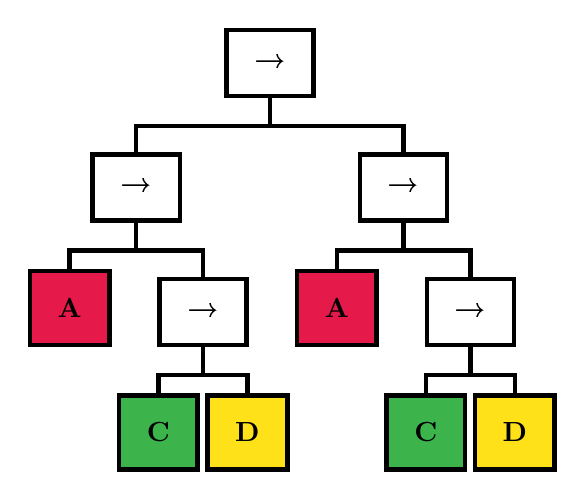
\begin{tikzpicture}

  \tikzstyle{ast} = [%
  align=center,
  draw=black,
  font=\bfseries,
  inner sep=10pt,
  line width=3pt,
  rectangle,
  ultra thick,
  ];

  \tikzset{level distance=45pt};
  \tikzset{edge from parent/.style=
    {
      draw,
      edge from parent path={(\tikzparentnode.south)
        -- +(0,-10pt)
        -| (\tikzchildnode.north)},
      ultra thick,
    }
  }

  \Tree
  [.\node[ast]{→};
    [.\node[ast]{→};
      [.\node[ast,fill=color01]{A}; ]
      [.\node[ast]{→};
        [.\node[ast,fill=color02]{C};]
        [.\node[ast,fill=color03]{D};]
      ]
    ]
    [.\node[ast]{→};
      [.\node[ast,fill=color01]{A}; ]
      [.\node[ast]{→};
        [.\node[ast,fill=color02]{C};]
        [.\node[ast,fill=color03]{D};]
      ]
    ]
  ]

\end{tikzpicture}

\begin{forest}
  for tree={
    align=center,
    draw=black,
    edge={
      ultra thick,
    },
    edge path={
      \noexpand\path[\forestoption{edge}]
      (!u.parent anchor)
      -- +(0,-10pt)
      -| (.child anchor)
      \forestoption{edge label};
    },
    font=\bfseries,
    %inner sep=10pt,
    %line width=2pt,
    minimum width=20pt,
    parent anchor=south,
    rectangle,
    ultra thick,
  }
  [→
    [→
      [A]
      [→ [C] [D]]
    ]
    [→
      [A]
      [→ [C] [D]]
    ]
  ]
\end{forest}


%\chapter{Related work}

\subsection*{Refactoring functional programs}

A main line of work in refactoring functional programs is the work done on the
Hare refactoring tool for \Haskell{}~\citep{li2005haskell} and subsequently on
refactoring Erlang programs~\citep{li2006}.  The scope of the former is much
larger than this paper: they implement a large library of refactoring
algorithms, including some that this paper covers, for the \Haskell{}
programming language.  In particular, their tool handles \Haskell{} 98, and
provides an API to perform refactorings.  They also refactor while preserving
the user's syntactic choices, which proves challenging in layout-based languages
like \Haskell{}.  However, their publications do not distill the details of how
to implement those refactorings, and thus, does not allow for easy
experimentation, porting to other languages, or verification of their
techniques.

A very promising ongoing line of work is that of
\define{ornaments}~\citep{williams2017}.  Their formalism allows to describe
data type transformations from within the language itself, and perform similar
transformations to ours.  The ornamentation language is more expressive than our
language of diffs in many ways, allowing arbitrary mappings between constructors
before and after modification: for instance, one of their motivating example
cuts a constructor into two different constructors depending on some Boolean
condition.  As a result, their technique requires the programmer to describe the
transformation they wish to carry as an ornament, and the programmer's help is
required alongside the transformation to indicate to the repair algorithm what
to do in corner cases.  Our restriction to a simple language of modifications
allows us to guess the transformation based on the syntactic modification of the
program itself, and grants us more leverage on automation, at the price of a
much lower expressiveness.

\subsection*{Refactoring proofs}

One of the few tools that attempts refactoring in the context of the proof
assistants is the Levity tool by~\citet{ruegenberg2011}.  The refactoring it
performs is referred to as \define{levitation}, and corresponds to the move of a
lemma up its dependency chain, to a location that is deemed more relevant.  This
transformation is hard to perform in many proof assistants, because figuring out
where the lemma can exist can be challenging and time-consuming, and because the
action of levitating the lemma might derail other parts of the proof
development, even when they seem unrelated, because the declaration of a lemma
might have unintended side-effects through automation mechanisms.

Another main line of work in this domain is the line of work
of~\citet{whiteside2011}, followed up by~\citet{dietrich2013}.  They define a
framework for specifying refactoring rules over an idealized proof language
called Hiproof, and its idealized tactic language called Hitac.  The latter is
designed to be close to the declarative Isar tactic language of Isabelle.  This
framework allows them to define many interesting refactorings, and to prove
their correctness, informally, with low effort.  They acknowledge that it would
be more difficult to develop the same refactorings for a less declarative tactic
language like the \Ltac{} language of the \Coq{} proof assistant.

\citet{boite2004} also addresses the problem of modifying an existing inductive
type definition while reusing existing proofs.  Their technique does not alter
existing code, rather, they internalize the notion of \define{extension} of an
inductive data type (that is, the adding of a constructor, or parameters), and
provide commands that perform such extensions, deriving extended data types and
extended functions from the original ones.  It would be interesting to have
proof assistants internalizing and exposing this kind of algebraic manipulations
of data types.

Finally, recent work by~\citet{ringer2018adapting} builds semantic patches to
help programmer refactor their proofs.  Their approach does not modify the old
program into a new program.  Rather, the old program is kept with its proofs,
alongside the new program, and patches are automatically derived to transport
proof obligations between the old program and the new program.  Their approach
seems complementary to ours, depending on the use case for the programmer.

\subsection*{Automatic code generation}

Another exciting line of work consists in removing the friction of performing
those manual refactorings altogether.

General purpose automation like Isabelle's sledgehammer~\citet{blanchette2011}
or the recent for on a similar hammer for Coq~\citet{czajka2017} can help reduce
the work of programmers in those systems by avoiding writing terms entirely.
Hopefully, doing so removes a lot of brittle tactic calls, but they do not help
in refactoring data type definitions when the objects of discourse evolve.

The body of work on program synthesis could also prove very beneficial.  For
instance,~\cite{polikarpova2016} can perform program synthesis from refinement
types, which could potentially spare the programmer from fixing code that is
never manually-written, but rather synthesized.  However, the specifications
themselves could still require refactoring tools, since they are themselves
terms from a refinement type system.

\subsection*{IDE-based detection of refactoring attempts}

The work of~\citet{foster2012} focuses on detecting when a programmer is trying
to perform a refactoring in Java programs.  Many times, the programmer will not
know that refactoring tools exist in their IDE, or will not realize that they
are performing a task that corresponds to an existing refactoring algorithm.  In
particular, they use a text-based diff in order to be able to recognize
refactoring attempts even when the program is in a transient, non-parseable
state.

\subsection*{Incremental computation}

The literature on incremental computation focuses on the problem of reliably and
efficiently re-computing data that is the output of some computation after the
input undergoes a modification, which is similar to our deriving of repairing
functions from Section~\ref{deriving}.  For instance,~\citet{acar2006},
\citet{carlsson2002}, as well as~\citet{firsov2016}, all use an abstract data
type for values that can be efficiently recomputed, and propose a monadic
interface to build incremental computations while providing the programmer with
an interface that hides those details behind the scenes.  Similarly,
\citet{chen2011} automatically transform a non-incremental program to inject
incremental behavior into it.  While this is similar to what we do in spirit,
we care about more than just obtaining the result of the incremental
computation, since we sometimes reuse the diff of one data type to compute a diff
for another, related data type.  Incremental computation techniques are
typically not interested in this, and do not usually expose the internals of
their functioning to the user.

\citet{cai2014} define a general way of using \define{derivatives} of functions
to compute their reactions to some abstract modifications, and compute those
derivatives for first-order functions.  They demonstrate it on examples using
unordered collections.  Our diffs are an instance of their general notion, but
we depart from it by having more specialized diffs to fit our needs, and by
supporting a small family of higher-order functions (namely, folds over lists),
using our deriving technique to help compute their derivative.


% \section*{HaRe: a \Haskell{} refactoring tool}

% \mycite{li2005haskell} propose a refactoring tool for \Haskell{} programs that
% provide several of the benefits of the tool we describe in
% Chapter~\ref{chick}.

% %TODO

% \section*{Ornaments}

% In order to refactor functional programs, as well as enabling novel methods of
% programming with data types, the work on \define{ornaments} approaches the
% treatment of programs as mathematical objects that can be related algebraically.

% \mycite{dagand2017essence} describes a theoretical framework for describing data
% types in such a way as to be able to express relationships between two data type
% definitions.  By representing inductive data type definitions with their
% underlying many-sorted signature, their work allows describing the relationship
% between two data types, describing one as an extension of the signature of the
% other one.  \mycite{williams2014ornaments} show how to use ornaments to perform
% a refactoring in which a data type representation gets reorganized without
% adding or removing information.

% Their approach is much more general and structured than ours: their work can
% effectively lift existing code through ornaments, or be used to express the
% relationship between a surface language and its syntactically-desugared version
% as an ornament.  However, this power comes with a price: first, the programmer
% must write their refactoring attempt in terms of an ornament, and then, they
% must participate in the lifting process by indicating to the algorithm what to
% do in some corner cases.  In our approach, the limited expressiveness of our
% diffs allows an algorithm to perform guesses as to what changed between two
% definitions, relieving the user from having to specify it.  We do, however, have
% similar limitations to our algorithm's ability to deal with ambiguous
% refactoring attempts, and we also rely on typed holes to fill blanks where the
% programmer must provide values to finish the generated code.

% \section*{Patching proof terms}

% \mycite{ringer2018adapting} propose a technique for automatically inferring
% proof patches based on an example of one patch.  This proves invaluable in
% refactoring settings, where a user might need to repeatedly apply the same
% repairing technique to several places in a code base.  By semantically analyzing
% one instance of such a repair, and performing abstraction techniques to make the
% repair more general, they can yield a patch that can be instantiated in many
% places to carry out the refactoring.

% Their current prototype does not support changes that don't preserve shape yet,
% so they could not be patching examples that ornaments and our technique handles.
% Their technique seems orthogonal to ours, since their intent is to obtain the
% new, patched proof as a proof term with the correct type, not as a repaired
% tactic script.  For repairing programs, this is similar, but for repairing
% proofs, their approach would yield a repaired proof object, but not a repaired
% proof text.  With our approach, we'd hope to be able to give tactic repairs, at
% the syntax level.

% However, the great advantage of their approach comes from the ability to find
% semantic, meaningful patches from examples.  While this requires some work from
% the user, they hope that the time saved by applying the patch repeatedly overall
% outweighs the time investment.


%\chapter{Takeaways}

\appendix

%\chapter{\PeaCoq{}}~\label{appendix-peacoq}

\section{\PeaCoq{} A-B study material}~\label{appendix-peacoq-material}

In this section, we report the entire listing of exercises provided to the participants of the A-B study described in Section~\ref{peacoq-a-b-study}.

\begin{minted}[fontsize=\scriptsize]{coq}
(* The following material is derived from Software Foundations by Benjamin
Pierce et al. Their work is under the following MIT license: *)

(*
Copyright (c) 2012

Permission is hereby granted, free of charge, to any person obtaining a copy
of this software and associated documentation files (the "Software"), to deal
in the Software without restriction, including without limitation the rights
to use, copy, modify, merge, publish, distribute, sublicense, and/or sell
copies of the Software, and to permit persons to whom the Software is
furnished to do so, subject to the following conditions:

The above copyright notice and this permission notice shall be included in
all copies or substantial portions of the Software.

THE SOFTWARE IS PROVIDED "AS IS", WITHOUT WARRANTY OF ANY KIND, EXPRESS OR
IMPLIED, INCLUDING BUT NOT LIMITED TO THE WARRANTIES OF MERCHANTABILITY,
FITNESS FOR A PARTICULAR PURPOSE AND NONINFRINGEMENT. IN NO EVENT SHALL THE
AUTHORS OR COPYRIGHT HOLDERS BE LIABLE FOR ANY CLAIM, DAMAGES OR OTHER
LIABILITY, WHETHER IN AN ACTION OF CONTRACT, TORT OR OTHERWISE, ARISING FROM,
OUT OF OR IN CONNECTION WITH THE SOFTWARE OR THE USE OR OTHER DEALINGS IN
THE SOFTWARE.
 *)

(* ###################################################################### *)
(** ** Days of the Week *)

Inductive day : Type :=
| monday : day
| tuesday : day
| wednesday : day
| thursday : day
| friday : day
| saturday : day
| sunday : day
.

Definition tomorrow (d: day) : day :=
  match d with
  | monday    => tuesday
  | tuesday   => wednesday
  | wednesday => thursday
  | thursday  => friday
  | friday    => saturday
  | saturday  => sunday
  | sunday    => monday
  end.

Theorem test_tomorrow:
  tomorrow saturday = sunday.
Proof.
  simpl. reflexivity.
Qed.

(* ###################################################### *)
(** ** Lists of Numbers *)

Inductive natlist : Type :=
| nil  : natlist
| cons : nat -> natlist -> natlist
.

Definition empty_list := nil.

Definition singleton_list := cons 42 nil.

Definition one_two_three := cons 1 (cons 2 (cons 3 nil)).

Fixpoint concat (l1 l2 : natlist) : natlist :=
  match l1 with
  | nil      => l2
  | cons h t => cons h (concat t l2)
  end.

Theorem test_concat1:
  concat (cons 1 (cons 2 nil))
         (cons 3 (cons 4 nil))
  = (cons 1 (cons 2 (cons 3 (cons 4 nil)))).
Proof.
  simpl. reflexivity.
Qed.

(* ###################################################### *)
(** * Reasoning About Lists *)

Theorem concat_nil_left : forall l : natlist,
  concat nil l = l.
Proof.
  (* FILL IN HERE *)
Qed.

Theorem concat_nil_right : forall l : natlist,
  concat l nil = l.
Proof.
  (* FILL IN HERE *)
Qed.

(* In-class exercise! *)
Theorem concat_associativity : forall l2 l1 l3 : natlist,
  concat (concat l1 l2) l3 = concat l1 (concat l2 l3).
Proof.
  (* FILL IN HERE *)
Qed.

(*
  [snoc] adds an element [v] at the end of the list [l]:
    snoc (cons 1 (cons 2 nil)) 3 = cons 1 (cons 2 (cons 3 nil))
*)
Fixpoint snoc (l: natlist) (v: nat) : natlist :=
  match l with
  | nil      => cons v nil
  | cons h t => cons h (snoc t v)
  end.

(*
  [rev] reverses a list:
    rev (cons 1 (cons 2 nil)) = cons 2 (cons 1 nil)
*)
Fixpoint rev (l: natlist) : natlist :=
  match l with
  | nil      => nil
  | cons h t => snoc (rev t) h
  end.

(* ###################################################### *)
(**
  For each theorem:
  - Discuss the statement of the theorem with your partner.
  - Once you understand it, prove the theorem.

  Every time you solve a theorem, switch who uses the keyboard/mouse.
 *)

Theorem rev_snoc : forall x l,
  rev (snoc l x) = cons x (rev l).
Proof.
  (* FILL IN HERE *)
Qed.

Theorem rev_involutive : forall l : natlist,
  rev (rev l) = l.
Proof.
  (* FILL IN HERE *)
Qed.

Theorem concat_cons_snoc : forall l1 x l2,
  concat l1 (cons x l2) = concat (snoc l1 x) l2.
Proof.
  (* FILL IN HERE *)
Qed.

(* ###################################################### *)

Module LogicExercises.

(* We now use notations from logic:
  /\   stands for the logical conjunction (AND) of two propositions
  \/   stands for the logical disjunction (OR)  of two propositions

  New tactics: left, right

  When your goal looks like [A \/ B]
  You get to pick which of [A] or [B] you will prove.
  If you believe you can prove [A], use the [left.] tactic.
  If you believe you can prove [B], use the [right.] tactic.

  Here is an example:
*)

Theorem goright_example : 0 = 1 \/ 1 = 1.
Proof. right. reflexivity.
Qed.

Theorem go_somewhere : 0 = 1 \/ (2 = 2 \/ 2 = 3).
Proof.
  (* FILL IN HERE *)
Qed.

(*
  New tactic: apply

  If you ever have a goal [G]
  And a hypothesis [H : G] or [H : X -> ... -> G]
  You can use the tactic [apply H.] to solve your goal in the former case,
  or turn your goal into subgoal(s) [X], [...] in the latter case.
*)

Theorem B_is_enough : forall A B : Prop,
  B ->
  A \/ B.
Proof.
  (* FILL IN HERE *)
Qed.

(*
  New tactic: split

  When your goal looks like [A /\ B]
  You need to prove both [A] and [B].
  The tactic [split.] lets you split your goal into these two goals.

  Here is an example:
*)

Theorem two_facts : nil = nil /\ 42 = 42.
Proof. split. reflexivity. reflexivity.
Qed.

Theorem more_facts : 1 = 2 \/ (1 = 1 /\ nil = nil).
Proof.
  (* FILL IN HERE *)
Qed.

Theorem A_and_B : forall A B : Prop,
  A ->
  B ->
  A /\ B.
Proof.
  (* FILL IN HERE *)
Qed.

End LogicExercises.

(* ###################################################### *)

Theorem snoc_concat_end : forall (l: natlist) (n: nat),
  snoc l n = concat l (cons n nil).
Proof.
  (* FILL IN HERE *)
Qed.

Theorem rev_distributes_over_concat : forall l1 l2 : natlist,
  rev (concat l1 l2) = concat (rev l2) (rev l1).
Proof.
  (* FILL IN HERE *)
Qed.

(* ###################################################### *)
(** We now introduce [map], which applies a function [f] to
    every element of a list [l].
*)

Fixpoint map (f: nat -> nat) (l: natlist) :=
  match l with
  | nil => nil
  | cons x xs => cons (f x) (map f xs)
  end.

Theorem map_commutes : forall f g l,
  (forall x, f (g x) = g (f x)) ->
  map f (map g l) = map g (map f l).
Proof.
  (* FILL IN HERE *)
Qed.

(* In this theorem, "fun x =>" introduces an anonymous function which receives
   a parameter [x] and returns the result on the right of the arrow. *)
Theorem map_fusion : forall f g l,
  map f (map g l) = map (fun x => f (g x)) l.
Proof.
  (* FILL IN HERE *)
Qed.

(* ###################################################### *)
(** We now introduce [fold], which processes a list with an
    accumulating function [f], starting from an initial value [b].
*)
Fixpoint fold (f: nat -> natlist -> natlist) (l: natlist) (b: natlist) :=
  match l with
  | nil => b
  | cons x xs => f x (fold f xs b)
  end.

Theorem fold_snoc : forall f l x b,
  fold f (snoc l x) b = fold f l (f x b).
Proof.
  (* FILL IN HERE *)
Qed.

Definition map' f l := fold (fun x fxs => cons (f x) fxs) l nil.

(* We use [Lemma] instead of [Theorem] here to indicate that this theorem may
   help you in proving the next theorem. *)
Axiom map'_unroll : forall f x xs,
  map' f (cons x xs) = cons (f x) (map' f xs).

Axiom map'_nil : forall f, map' f nil = nil.

Theorem map_map' : forall f l, map f l = map' f l.
Proof.
  (* FILL IN HERE *)
Qed.

Ltac cases H := match type of H with _ \/ _ => destruct H end.

(*
  New tactics: cases, contradiction

  When a hypothesis looks like [H : A \/ B]
  You have to prove the goal for each case, to do so, use the tactic [cases H.]
  You will get two goals as a result, one with a [A] hypothesis, one with a [B] hypothesis.

  Finally, if you ever get a hypothesis like [H : False]
  You have derived a contradiction, and you can indicate this to the system by calling
  the tactic [contradiction.], which will solve your goal.
*)

Fixpoint In n l :=
  match l with
  | nil      => False
  | cons h t => h = n \/ In n t
  end.

Theorem In_cons : forall x h l,
  In x l ->
  In x (cons h l).
Proof.
  (* FILL IN HERE *)
Qed.

(*
  New tactic: simpl in *

  Sometimes, you might want to simplify things in your hypotheses, the same way things
  can be simplified in your conclusion.
*)

Theorem In_concat_left : forall x l1 l2,
  In x l1 ->
  In x (concat l1 l2).
Proof.
  (* FILL IN HERE *)
Qed.
\end{minted}

\clearpage

\section{\PeaCoq{} A-B study post-study survey}~\label{appendix-peacoq-a-b-study}

We report the qualitative feedback obtained via a questionnaire given after the
A-B study described in Section~\ref{peacoq-a-b-study}.  We indicate participants
anonymously as $Xp_{i}$ where $X$ stands for the study group ($A$ being the
\define{control group}, $B$ being the group testing our tool), $p$ stands for a
given pair of participants, and $i$ distinguishes between the two participants
in a pair.

We report participants' answers as is: we do fix typos, but do not alter their
phrasing or grammatical structures whatsoever.

\clearpage

\noindent
\begin{tabularx}{\linewidth}{@{}cX@{}}
  \toprule
  Participant & \multicolumn{1}{c}{
    \textbf{In your own words, describe what you did today.}
  } \\ \midrule
  $A1_{1}$ & Proved several theorems in a pair using an interactive proof assistant. \\
  $A1_{2}$ & \begin{enumerate} \item Proved some set and logic and operation lemmas and theorems. \item Used a new tool to write the proofs. \end{enumerate} \\
  $A2_{1}$ & Tried to understand \Coq{} by using an entire IDE and write some proofs. \\
  $A2_{2}$ & We used a proof assistant to prove theorems about lists and their properties. \\
  $A3_{1}$ & We used the theorem prover to prove that the functions of code did what they meant to in all cases. \\
  $A3_{2}$ & Today I learned about the \Coq{} theorem proving language.  After an introduction, I worked in a pair to solve various theorems for lists of natural numbers, and maps. \\
  $A4_{1}$ & Use an automated theorem prover to prove basic facts in data structures and logic. \\
  $A4_{2}$ & We used a tool that could define predicates, types and prove various properties about them. \\
  $A5_{1}$ & We learned a little about basic proofs in \Coq{} then applied what we learned in the exercises. \\
  $A5_{2}$ & I used a proof assistant to prove several simple mathematical theorems. \\
  \bottomrule
\end{tabularx}{\parfillskip=0pt\par}

\clearpage

\noindent
\begin{tabularx}{\linewidth}{@{}cX@{}}
  \toprule
  Participant & \multicolumn{1}{c}{
    \textbf{In your own words, describe what you did today.}
  } \\ \midrule
  $B1_{1}$ & I used a graphical tool to prove several invariants about functions/data structures in a given language (\Coq{}). \\
  $B1_{2}$ & Proved some special cases of inferences from new definitions using induction and other primitive proof techniques.  Use already proved theorems in future proofs. \\
  $B2_{1}$ & I used a programming language tool to prove various constructs. \\
  $B2_{2}$ & Proved a bunch of simple theorems about functions working on lists. \\
  $B3_{1}$ & Use \Coq{} to prove a theorem.  Reasoning the steps and select what makes sense from the options given by the tool. \\
  $B3_{2}$ & We were trying to use \PeaCoq{} to prove a bunch of theorems by exploring all the possible strategies, such as induction, transformation, simplification, etc. \\
  $B4_{1}$ & We used a graphical version of an interactive proof assistant to prove some theorems involving list operations. \\
  $B4_{2}$ & Proved some functions using \PeaCoq{}. \\
  $B5_{1}$ & We used the \PeaCoq{} web editor interface to prove theorems on pieces of code via \Coq{}.  First we were given an introduction to \Coq{} combined with a tutorial on using the tool, and then we worked in pairs on a series of example of proofs/theorems. \\
  $B5_{2}$ & I used a modified version of the \Coq{} proof assistant to prove things about lists and functions over them. \\
  \bottomrule
\end{tabularx}{\parfillskip=0pt\par}

\clearpage

\noindent
\begin{tabularx}{\linewidth}{@{}cX@{}}
  \toprule
  Participant & \multicolumn{1}{c}{
    \textbf{What did the experience today remind you of?}
  } \\ \midrule
  $A1_{1}$ & Learning to program for the first time. Lots of brute-forcing and trying things that worked in the past to see if they would work in a new context. \\
  $A1_{2}$ & Using induction in high school/undergrad and trying to draw insights from proving the base case to apply to the general case. \\
  $A2_{1}$ & Today was quite unique but I felt like writing functional programs since I tried to prove my implementation there too. \\
  $A2_{2}$ & It reminded me of working on large code bases where certain things appear to work by magic.  Fixes/proofs were performed with little fundamental understanding. \\
  $A3_{1}$ & Taking a programming languages class, since the constructs are all the same. \\
  $A3_{2}$ & Today's experience reminded me of an intro to algorithms course. \\
  $A4_{1}$ & Proving mathematical theorems for research. \\
  $A4_{2}$ & Liquid types in Haskell.  Mathematical induction. \\
  $A5_{1}$ & Learning programming in school and proofs in math classes. \\
  $A5_{2}$ & It reminded me of pen-and-paper proofs. \\
  \bottomrule
\end{tabularx}{\parfillskip=0pt\par}

\clearpage

\noindent
\begin{tabularx}{\linewidth}{@{}cX@{}}
  \toprule
  Participant & \multicolumn{1}{c}{
    \textbf{What did the experience today remind you of?}
  } \\ \midrule
  $B1_{1}$ & Playing a logical/exploration game. \\
  $B1_{2}$ & \begin{enumerate} \item Writing unit tests for corner cases. \item Giving a systematic proof covering all cases. \end{enumerate} \\
  $B2_{1}$ & It reminded me of safe programming techniques in the way that if we can prove that our constructs work, there shouldn't be any problems at run-time. \\
  $B2_{2}$ & Functional programming and reasoning about it. \\
  $B3_{1}$ & First time to learn formal proof stuff. \\
  $B3_{2}$ & Decision tree. \\
  $B4_{1}$ & It reminded me of a puzzle game in which you have to reach a target and can use as keys some of the facts you encounter on your way there. \\
  $B4_{2}$ & Proving technique classes. \\
  $B5_{1}$ & The \inferrule{ \text{rules} \\\\ \text{rules} \\\\ \text{rules} }{ statement } format reminded me of constructions I have seen in computer science papers that have not formally learned about.  The theorems we were proving, e.g. \safecoqinline{concat xs nil = xs}, reminded in a different/more powerful direction (but requiring manual work to prove). \\
  $B5_{2}$ & Analysis class, proving simple-seeming things about math was similarly harder than it looked. \\
  \bottomrule
\end{tabularx}{\parfillskip=0pt\par}

\clearpage

\noindent
\begin{tabularx}{\linewidth}{@{}cX@{}}
  \toprule
  Participant & \multicolumn{1}{c}{
    \textbf{Did you understand all the proofs you completed?}
  } \\ \midrule
  $A1_{1}$ & No. \\
  $A1_{2}$ & No.  We figured out that there were some hammers which we should keep using (\safecoqinline{simpl}, \safecoqinline{reflexivity}, \safecoqinline{rewrite}).  They mostly made sense but we didn't spend time to understand the exact changes they made. \\
  $A2_{1}$ & Most of them.  Especially the last ones were quite confusing. \\
  $A2_{2}$ & Not entirely.  While I had conceptual knowledge of what was happening, I didn't understand it holistically. \\
  $A3_{1}$ & Yes. \\
  $A3_{2}$ & Yes. \\
  $A4_{1}$ & Yes. \\
  $A4_{2}$ & Yes. \\
  $A5_{1}$ & Yes. \\
  $A5_{2}$ & Yes. \\
  \bottomrule
\end{tabularx}{\parfillskip=0pt\par}

\clearpage

\noindent
\begin{tabularx}{\linewidth}{@{}cX@{}}
  \toprule
  Participant & \multicolumn{1}{c}{
    \textbf{Did you understand all the proofs you completed?}
  } \\ \midrule
  $B1_{1}$ & Yes. \\
  $B1_{2}$ & Yes. \\
  $B2_{1}$ & Yes, the only one that I had trouble with was \safecoqinline{destruct}. \\
  $B2_{2}$ & No. \\
  $B3_{1}$ & No.  Sometimes it is magically done. \\
  $B3_{2}$ & No, but most of them. \\
  $B4_{1}$ & Yes (at least on a second closer inspection). \\
  $B4_{2}$ & No. \\
  $B5_{1}$ & For the most part.  The last exercise (\safecoqinline{In_concat_left}) had me a bit confused on how \safecoqinline{destruct} worked/what it did.  Once that clicked for me, what we were doing there made sense. \\
  $B5_{2}$ & I think so? \\
  \bottomrule
\end{tabularx}{\parfillskip=0pt\par}

\clearpage

\noindent
\begin{tabularx}{\linewidth}{@{}cX@{}}
  \toprule
  Participant & \multicolumn{1}{c}{
    \textbf{Did you find the tool useful for achieving the tasks?}
  } \\ \midrule
  $A1_{1}$ & Error messages were mostly helpful sometimes. Sort of. Clear when something didn't work. \\
  $A1_{2}$ & Yes.  Because it would stop me from trying to use wrong rules.  Also because I could follow from one lemma to another in most cases. \\
  $A2_{1}$ & \begin{enumerate} \item Has a simple, clean UI, \item Doesn't require anything other than a browser. \end{enumerate} \\
  $A2_{2}$ & A little.  It provided confidence that the task was completed correctly. \\
  $A3_{1}$ & Yes.  I like how the right side always showed the next goal, in that it was easy to focus on one statement at a time. \\
  $A3_{2}$ & Yes, very. \\
  $A4_{1}$ & Yes, it was pretty self-explanatory.  Inline code and comments very helpful. \\
  $A4_{2}$ & Yes. \\
  $A5_{1}$ & Yes, the step by step approach was helpful to visualize how the proof was coming along.  It also helped with trial and error. \\
  $A5_{2}$ & Highlighting, previous/next were extremely useful.  The information snippets would be useful if I weren't the proof author. \\
  \bottomrule
\end{tabularx}{\parfillskip=0pt\par}

\clearpage

\noindent
\begin{tabularx}{\linewidth}{@{}cX@{}}
  \toprule
  Participant & \multicolumn{1}{c}{
    \textbf{Did you find the tool useful for achieving the tasks?}
  } \\ \midrule
  $B1_{1}$ & The tool was very useful, specifically: \begin{enumerate} \item Highlighting the diffs was helpful to explain what each tactic does, \item Having all the options available to apply was helpful for a novice who doesn't know what the available tactics are. \end{enumerate} \\
  $B1_{2}$ & Yes. \\
  $B2_{1}$ & It definitely helped in showing the paths you could take in a proof, which is helpful if you can't think of them on the spot. \\
  $B2_{2}$ & I proved things without having to think too hard about it. \\
  $B3_{1}$ & \begin{enumerate} \item As an inexperienced learner, I even don't know how to start a proof, but the tool gives me the guidance to do this. \item After some time, when you get familiar with it, there exists some patterns to find the correct solution. \end{enumerate} \\
  $B3_{2}$ & I think it's useful.  But it is hard to say ``how'' useful it is for two reasons: \begin{enumerate} \item I'm not aware of any order tools, \item the problems are actually simple and intuitive to prove manually. \end{enumerate} \\
  $B4_{1}$ & \begin{enumerate} \item Provided a broad overview of the available options (some perhaps ``counter-intuitive'' options that I might have thought of were presented right away), \item fewer keystrokes \item visual diffs are very useful for calculating how bigger / smaller our target is. \end{enumerate} \\
  $B4_{2}$ & I wouldn't be able to achieve the tasks on my own, but that's probably because I have no idea how to prove those things. \\
  $B5_{1}$ & Yes, absolutely.  The tree interface made exploring possible tactics and seeing the results very quick and easy.  I've never actually used \Coq{} or anything like it before but with this interface I was able to get up to speed pretty quickly. \\
  $B5_{2}$ & I didn't have to already know/remember the set of options, and it was useful to get a preview of what each one would do. \\
  \bottomrule
\end{tabularx}{\parfillskip=0pt\par}

\clearpage

\noindent
\begin{tabularx}{\linewidth}{@{}cX@{}}
  \toprule
  Participant & \multicolumn{1}{c}{
    \textbf{Do you have suggestions on how to improve the tool you used today?}
  } \\ \midrule
  $A1_{1}$ & Backing up through a \safecoqinline{Qed.} backs up the entire proof.  Would prefer to step back one tactic at a time like during the proof.  Right-hand pane sometimes not wide enough to see everything.  Primitive sub-string matching to suggest rewrites would be useful. \\
  $A1_{2}$ & \begin{enumerate} \item It should stop me from going down useless proof steps even though the rules apply. \item It should stop me from going in circles by warning (we are not sure we did that but came close). \item Difficult to translate intuition from base case to general case.  Had to use pen-and-paper at times to write small examples. \end{enumerate} \\
  $A2_{1}$ & \begin{enumerate} \item Missing some keyboard shortcuts. \item Having a pane which shows previous proofs would be quite helpful. \end{enumerate} \\
  $A2_{2}$ & I had little confidence that I understood what was happening.  Completing the same proofs later would likely result in similar trial and error.  The only thing I was learning was the sort of patterns that proofs took on.  Variable names were confusing and hard to work with. \\
  $A3_{1}$ & \safecoqinline{each} should be syntax-highlighted. \\
  $A3_{2}$ & Adding auto-complete would be nice and a command list. \\
  $A4_{1}$ & Previously proved functions were difficult to find/see when scrolling up.  I could see this being a major problem for anything complex.  Could be solved with a better interface e.g.\ in an IDE.\@Not related to the software, but there's a tendency to avoid planning and just react to results of \safecoqinline{simpl}, \safecoqinline{rewrite}, etc. \\
  $A4_{2}$ & \begin{enumerate} \item Bugs when we were using Firefox instead of Chrome.  Tool wouldn't revert steps correctly. \item Auto-completion of previously defined rewrite theorems \end{enumerate} \\
  $A5_{1}$ & Flip Next and Previous in the GUI. \\
  $A5_{2}$ & Some sort of search (``I want to use this'') would be handy.  The coloring breaks on exceptions. \\
  \bottomrule
\end{tabularx}{\parfillskip=0pt\par}

\clearpage

\noindent
\begin{tabularx}{\linewidth}{@{}cX@{}}
  \toprule
  Participant & \multicolumn{1}{c}{
    \textbf{Do you have suggestions on how to improve the tool you used today?}
  } \\ \midrule
  $B1_{1}$ & \begin{enumerate} \item Highlight the border of the sub-window (code/proof) that has keyboard focus, \item When deep in a proof tree, I kept forgetting what induction hypothesis I had accumulated so far (and I think I didn't always see them in the current goal).  It would be useful to somehow get reminded of what invariants/induction hypothesis I had accumulated. \end{enumerate} \\
  $B1_{2}$ & A first time user might find it difficult to switch between cases using ``['' and ``]''.  Some syntax in languages were not straightforward, for instance \safecoqinline{fold}.  Syntax of \safecoqinline{map} functions were clear. \\
  $B2_{1}$ & Maybe look ahead and see if some paths don't lead to solutions. \\
  $B2_{2}$ & \emph{No answer provided.} \\
  $B3_{1}$ & \emph{No answer provided.} \\
  $B3_{2}$ & I guess it's definitely helpful if the tool can automatically probing some paths without clicking. \\
  $B4_{1}$ & \begin{enumerate} \item Trivialize options that lead to the target in one to two steps. \item On the fly explanation of what the operators do. \end{enumerate} \\
  $B4_{2}$ & It crashes when you hit the left button three or four times quickly. \\
  $B5_{1}$ & There was that one bug that we ran into a few times: going back causing the editor to crash, that made us lose progress a few times.  \begin{enumerate} \item An auto-save feature would be appreciated as a guard against this (could use e.g. Local Storage API), \item A way to ``bookmark'' and jump back to points in the tree would be appreciated, perhaps also some highlights of previously explored paths? \end{enumerate} \\
  $B5_{2}$ & A minor one: \safecoqinline{intros.} should be option one (instead of \safecoqinline{intro x.}) since it always seems like the right start. \\
  \bottomrule
\end{tabularx}{\parfillskip=0pt\par}

\clearpage

\noindent
\begin{tabularx}{\linewidth}{@{}cX@{}}
  \toprule
  Participant & \multicolumn{1}{c}{
    \textbf{Explain in your own word what the \safecoqinline{each} tactic does.}
  } \\ \midrule
  $A1_{1}$ & Splits up an \safecoqinline{AND} so each side can be proven separately. \\
  $A1_{2}$ & Split/divides a proof of an \safecoqinline{AND} expression into two different proof exercises. \\
  $A2_{1}$ & Used to prove both paths of a theorem (conjunction) with two parts. \\
  $A2_{2}$ & Splits a logical \safecoqinline{and} into subgoals for each expression. \\
  $A3_{1}$ & Follow both branches of an \safecoqinline{AND}, since both must be proven. \\
  $A3_{2}$ & Selects the terms from both sides of an \safecoqinline{AND}. \\
  $A4_{1}$ & Enumerates all cases in a conjunction. \\
  $A4_{2}$ & Divides the \safecoqinline{AND} predicate into two sub-problems so we can prove each separately. \\
  $A5_{1}$ & Splits an \safecoqinline{and} into each side so they can be proved separately. \\
  $A5_{2}$ & Split conjunction. \\
  \bottomrule
\end{tabularx}{\parfillskip=0pt\par}

\clearpage

\noindent
\begin{tabularx}{\linewidth}{@{}cX@{}}
  \toprule
  Participant & \multicolumn{1}{c}{
    \textbf{Explain in your own word what the \safecoqinline{each} tactic does.}
  } \\ \midrule
  $B1_{1}$ & For a goal \safecoqinline{A /\ B} introduces 2 subgoals \safecoqinline{A} and \safecoqinline{B}. \\
  $B1_{2}$ & Prove each child tree is correct. \\
  $B2_{1}$ & Applies some function to all elements in a set. \\
  $B2_{2}$ & Prove all sub-trees. \\
  $B3_{1}$ & Every element in a collection. \\
  $B3_{2}$ & Try to prove each case. \\
  $B4_{1}$ & Apply action to all elements of a collection. \\
  $B4_{2}$ & ? \\
  $B5_{1}$ & When you have \safecoqinline{A /\ B}, you need to prove both \safecoqinline{A} and \safecoqinline{B}, so split, doing \safecoqinline{A} and then \safecoqinline{B}. \\
  $B5_{2}$ & Splits an \safecoqinline{A /\ B} goal into separate \safecoqinline{A} and \safecoqinline{B} goals. \\
  \bottomrule
\end{tabularx}{\parfillskip=0pt\par}

\clearpage

\noindent
\begin{tabularx}{\linewidth}{@{}cX@{}}
  \toprule
  Participant & \multicolumn{1}{c}{
    \textbf{Explain in your own word what the \safecoqinline{intro} tactic does.}
  } \\ \midrule
  $A1_{1}$ & Fixes some \safecoqinline{forall} value. \\
  $A1_{2}$ & Introduces the different variables in the expression. \\
  $A2_{1}$ & Instantiates the \safecoqinline{forall} variables. \\
  $A2_{2}$ & Do it first thing? \\
  $A3_{1}$ & Apply a \safecoqinline{foreach}. \\
  $A3_{2}$ & Provides the types for the theorem we are proving. \\
  $A4_{1}$ & Instantiates a placeholder variable under a universal quantifier. \\
  $A4_{2}$ & Infers already known information from the setup to give us known or assumed values. \\
  $A5_{1}$ & List names of variables in \safecoqinline{forall} and hypotheses. \\
  $A5_{2}$ & Instantiate \safecoqinline{forall}. \\
  \bottomrule
\end{tabularx}{\parfillskip=0pt\par}

\clearpage

\noindent
\begin{tabularx}{\linewidth}{@{}cX@{}}
  \toprule
  Participant & \multicolumn{1}{c}{
    \textbf{Explain in your own word what the \safecoqinline{intro} tactic does.}
  } \\ \midrule
  $B1_{1}$ & Given a \safecoqinline{forall x, p(x)} goal, make up a new variable name \safecoqinline{x} and introduce it and make \safecoqinline{p(x)} (with that specific \safecoqinline{x}) the current sub-goal. \\
  $B1_{2}$ & Introduce (or define) the variables used in proof. \\
  $B2_{1}$ & Introduces all the components of your proof in order to use them. \\
  $B2_{2}$ & Introduce quantified variables (i.e. give them a name). \\
  $B3_{1}$ & Extend the original theorem to an easy-to-understand format. \\
  $B3_{2}$ & Give a start point. \\
  $B4_{1}$ & Add facts to your assumptions. \\
  $B4_{2}$ & ? \\
  $B5_{1}$ & Take the names from the \safecoqinline{forall} and put them in the usable rule environment.  It was sort of unclear to me why we needed to do this explicitly every time. \\
  $B5_{2}$ & Equivalent of the mathematician's ``fix'', gets rid of \safecoqinline{forall}. \\
  \bottomrule
\end{tabularx}{\parfillskip=0pt\par}

\clearpage

\noindent
\begin{tabularx}{\linewidth}{@{}cX@{}}
  \toprule
  Participant & \multicolumn{1}{c}{
    \textbf{Explain in your own word what the \safecoqinline{induction} tactic does.}
  } \\ \midrule
  $A1_{1}$ & Allows case analysis over inductive types. \\
  $A1_{2}$ & Applies induction the variable mentioned as parameter and breaks the proof into base case and general case. \\
  $A2_{1}$ & To use induction on a given variable.  Proof by cases analysis. \\
  $A2_{2}$ & Perform induction with two steps/goals: base case + inductive case. \\
  $A3_{1}$ & Break a step into its base case(s) and recursive case(s). \\
  $A3_{2}$ & Performs induction on an element. \\
  $A4_{1}$ & Breaks a logical statement universally quantifying over a variable \safecoqinline{x}, into cases based on \safecoqinline{match}. \\
  $A4_{2}$ & Performs mathematical induction.  Divides into base case, induction case.  Assumes hypothesis. \\
  $A5_{1}$ & Breaks a list into the base case and induction step. \\
  $A5_{2}$ & Induct over recursive variable. \\
  \bottomrule
\end{tabularx}{\parfillskip=0pt\par}

\clearpage

\noindent
\begin{tabularx}{\linewidth}{@{}cX@{}}
  \toprule
  Participant & \multicolumn{1}{c}{
    \textbf{Explain in your own word what the \safecoqinline{induction} tactic does.}
  } \\ \midrule
  $B1_{1}$ & If \safecoqinline{x} is of a given type (like ML algebraic types), do a case analysis for each of the constructors of the type.  If one of them is recursive, introduce a hypothesis for its sub-part, and use it to prove the statement for the larger goal. \\
  $B1_{2}$ & Split into two branches: base case and induction case.  Introduce a hypothesis argument called \safecoqinline{IH} which can be invoked later in the proof. \\
  $B2_{1}$ & Proves that some function works for arbitrary element. \\
  $B2_{2}$ & Start an inductive proof (base case + step). \\
  $B3_{1}$ & \begin{enumerate} \item Base case, \item Induction... \end{enumerate} \\
  $B3_{2}$ & It's just ``induction'' we do... counting base case, inductive hypothesis, inductive steps. \\
  $B4_{1}$ & Do structural induction of a... \\
  $B4_{2}$ & Proof by induction. \\
  $B5_{1}$ & Case analysis: break e.g. a list into \safecoqinline{nil} and \safecoqinline{cons}, and branch along each path with an additional inductive hypothesis, proving each path (one for each possible value/case) proves the overall theorem. \\
  $B5_{2}$ & Splits a goal involving a recursively-defined data type into a base case and an inductive step goal (in the latter, you get the inductive hypothesis in the environment). \\
  \bottomrule
\end{tabularx}{\parfillskip=0pt\par}

\clearpage

\noindent
\begin{tabularx}{\linewidth}{@{}cX@{}}
  \toprule
  Participant & \multicolumn{1}{c}{
    \textbf{Explain in your own word what the \safecoqinline{reflexivity} tactic does.}
  } \\ \midrule
  $A1_{1}$ & Used when x = x. \\
  $A1_{2}$ & Comparing an expression with itself is true. \\
  $A2_{1}$ & Used to prove equality when both sides of the equality is the same (or very similar after simplifying). \\
  $A2_{2}$ & Attempt to reconcile an equality. \\
  $A3_{1}$ & When you have \safecoqinline{x = x}, call that step finished and move on to the next. \\
  $A3_{2}$ & Simplifies like expressions on both sides of the equality. \\
  $A4_{1}$ & Uses the tautological identity to prove trivial equalities.  Also does \safecoqinline{simpl}. \\
  $A4_{2}$ & \safecoqinline{A == A}. \\
  $A5_{1}$ & Simplifies and accepts if both sides are the same. \\
  $A5_{2}$ & Apply functions, find structural equality. \\
  \bottomrule
\end{tabularx}{\parfillskip=0pt\par}

\clearpage

\noindent
\begin{tabularx}{\linewidth}{@{}cX@{}}
  \toprule
  Participant & \multicolumn{1}{c}{
    \textbf{Explain in your own word what the \safecoqinline{reflexivity} tactic does.}
  } \\ \midrule
  $B1_{1}$ & \safecoqinline{x = x} is trivially true. \\
  $B1_{2}$ & \safecoqinline{a = a}.  Also simplifies based on definition of types. \\
  $B2_{1}$ & Two things are equivalent. \\
  $B2_{2}$ & Check if two things are equal. \\
  $B3_{1}$ & \safecoqinline{x = x}. \\
  $B3_{2}$ & Trivial equivalence. \\
  $B4_{1}$ & Use the reflexive property (along with some simplification). \\
  $B4_{2}$ & Checks if two things are the same. \\
  $B5_{1}$ & Prove \safecoqinline{a = a} for some \safecoqinline{a}. \\
  $B5_{2}$ & Proves \safecoqinline{x = x} (also performs simple simplifications). \\
  \bottomrule
\end{tabularx}{\parfillskip=0pt\par}

\clearpage

\noindent
\begin{tabularx}{\linewidth}{@{}cX@{}}
  \toprule
  Participant & \multicolumn{1}{c}{
    \textbf{Explain in your own word what the \safecoqinline{rewrite} tactic does.}
  } \\ \midrule
  $A1_{1}$ & Used to pull in some fact proven earlier. \\
  $A1_{2}$ & Uses the rule provided to find a component in LHS/RHS (depending on arrow) and modify it (as per the rule). \\
  $A2_{1}$ & Uses a rule to rewrite a part of the proof. \\
  $A2_{2}$ & Pattern-match and replace. \\
  $A3_{1}$ & Rewrite the current step with a specified function. \\
  $A3_{2}$ & Applies an equality to your current goal or sub-goal. \\
  $A4_{1}$ & Pattern-match part of an expression using a (inductive) hypothesis in scope. \\
  $A4_{2}$ & Substitution. \\
  $A5_{1}$ & Replaces one side of an expression with the other. \\
  $A5_{2}$ & Replace equal terms. \\
  \bottomrule
\end{tabularx}{\parfillskip=0pt\par}

\clearpage

\noindent
\begin{tabularx}{\linewidth}{@{}cX@{}}
  \toprule
  Participant & \multicolumn{1}{c}{
    \textbf{Explain in your own word what the \safecoqinline{rewrite} tactic does.}
  } \\ \midrule
  $B1_{1}$ & Use a previous lemma/induction hypothesis to transform some terms. \\
  $B1_{2}$ & Replace parts of LHS, RHS, using the theorems proved earlier. \\
  $B2_{1}$ & Use previous lemma or theorems to modify the construct. \\
  $B2_{2}$ & Use previously proven things to rewrite the expression. \\
  $B3_{1}$ & Rewrite some formulas to ones that are closer to the proof's target.  Better to utilize the existing hypothesis. \\
  $B3_{2}$ & Transformation. \\
  $B4_{1}$ & Use some rewrite property applied to parts of your expressions. \\
  $B4_{2}$ & Replaces a pattern in the text. \\
  $B5_{1}$ & Use a theorem/inductive hypothesis/other rewrite rule to transform part of the current node and continue with the proof. \\
  $B5_{2}$ & ``Substitution'' or ``plugging int''. \\
  \bottomrule
\end{tabularx}{\parfillskip=0pt\par}

\clearpage

\noindent
\begin{tabularx}{\linewidth}{@{}cX@{}}
  \toprule
  Participant & \multicolumn{1}{c}{
    \textbf{Explain in your own word what the \safecoqinline{goright} tactic does.}
  } \\ \midrule
  $A1_{1}$ & Tells proof assistant I'm about to prove the right-hand side of an \safecoqinline{OR}. \\
  $A1_{2}$ & Choose the right-side expression in a combination of Boolean expressions. \\
  $A2_{1}$ & To prove the right part of an \safecoqinline{OR} expression. \\
  $A2_{2}$ & Take a goal with a logical \safecoqinline{or} and solve only the right sub-expression. \\
  $A3_{1}$ & Follow the right branch of an \safecoqinline{OR}, ignoring the left. \\
  $A3_{2}$ & Selects the right side of a logical comparison. \\
  $A4_{1}$ & Try to prove the second clause in a disjunction. \\
  $A4_{2}$ & Discard left side of the \safecoqinline{or} predicate. \\
  $A5_{1}$ & Selects the right-hand side of an \safecoqinline{or} gate to try to prove. \\
  $A5_{2}$ & Follow right arm of disjunction. \\
  \bottomrule
\end{tabularx}{\parfillskip=0pt\par}

\clearpage

\noindent
\begin{tabularx}{\linewidth}{@{}cX@{}}
  \toprule
  Participant & \multicolumn{1}{c}{
    \textbf{Explain in your own word what the \safecoqinline{goright} tactic does.}
  } \\ \midrule
  $B1_{1}$ & Given a goal \safecoqinline{A \/ B} try to prove \safecoqinline{B}. \\
  $B1_{2}$ & While proving \safecoqinline{\/}, choose the right clause to prove. \\
  $B2_{1}$ & Choose the right hand goal of an \safecoqinline{OR} construct to continue a proof. \\
  $B2_{2}$ & Prove the right side of the \safecoqinline{\/} expression. \\
  $B3_{1}$ & Prove the right side. \\
  $B3_{2}$ & For \safecoqinline{A \/ B} or \safecoqinline{A /\ B}, try to prove the right proposition. \\
  $B4_{1}$ & Prove the right part of a disjunction. \\
  $B4_{2}$ & Visits the right-hand side of an \safecoqinline{OR} statement. \\
  $B5_{1}$ & When you have \safecoqinline{A \/ B}, you need to prove \safecoqinline{A} or \safecoqinline{B}, here, we choose to prove \safecoqinline{B} to prove the overall statement. \\
  $B5_{2}$ & Replaces \safecoqinline{A \/ B} goal with \safecoqinline{B}. \\
  \bottomrule
\end{tabularx}{\parfillskip=0pt\par}

\clearpage

\noindent
\begin{tabularx}{\textwidth}{ | c || *{6}{Y|} }
  \hline
  Participant & \multicolumn{5}{c|}{
    \textbf{I found the tool easy to understand.}
  } \\ \hline
  & \makecell{Strongly\\disagree} & Disagree & Neutral & Agree & \makecell{Strongly\\agree} \\ \hline
  $A1_{1}$ &   &   &   &   &\OK\\ \hline
  $A1_{2}$ &   &   &   &\OK&   \\ \hline
  $A2_{1}$ &   &   &   &\OK&   \\ \hline
  $A2_{2}$ &   &   &\OK&   &   \\ \hline
  $A3_{1}$ &   &   &   &\OK&   \\ \hline
  $A3_{2}$ &   &   &   &   &\OK\\ \hline
  $A4_{1}$ &   &   &   &   &\OK\\ \hline
  $A4_{2}$ &   &   &\OK&   &   \\ \hline
  $A5_{1}$ &   &   &   &   &\OK\\ \hline
  $A5_{2}$ &   &   &   &   &\OK\\ \hline \hline
  $B1_{1}$ &   &   &   &   &\OK\\ \hline
  $B1_{2}$ &   &   &   &\OK&   \\ \hline
  $B2_{1}$ &   &   &   &   &\OK\\ \hline
  $B2_{2}$ &   &   &   &\OK&   \\ \hline
  $B3_{1}$ &   &   &\OK&   &   \\ \hline
  $B3_{2}$ &   &   &   &   &\OK\\ \hline
  $B4_{1}$ &   &   &   &   &\OK\\ \hline
  $B4_{2}$ &   &\OK&   &   &   \\ \hline
  $B5_{1}$ &   &   &   &\OK&   \\ \hline
  $B5_{2}$ &   &   &   &   &\OK\\ \hline
\end{tabularx}{\parfillskip=0pt\par}

\clearpage

\noindent
\begin{tabularx}{\textwidth}{ | c || *{6}{Y|} }
  \hline
  Participant & \multicolumn{5}{c|}{
    \textbf{ I found the session educational. }
  } \\ \hline
  & \makecell{Strongly\\disagree} & Disagree & Neutral & Agree & \makecell{Strongly\\agree} \\ \hline
  $A1_{1}$ &   &   &   &   &\OK\\ \hline
  $A1_{2}$ &   &   &   &   &\OK\\ \hline
  $A2_{1}$ &   &   &   &   &\OK\\ \hline
  $A2_{2}$ &   &   &   &   &\OK\\ \hline
  $A3_{1}$ &   &   &   &   &\OK\\ \hline
  $A3_{2}$ &   &   &\OK&   &   \\ \hline
  $A4_{1}$ &   &   &   &\OK&   \\ \hline
  $A4_{2}$ &   &   &   &\OK&   \\ \hline
  $A5_{1}$ &   &   &   &   &\OK\\ \hline
  $A5_{2}$ &   &   &   &   &\OK\\ \hline \hline
  $B1_{1}$ &   &   &   &   &\OK\\ \hline
  $B1_{2}$ &   &   &   &\OK&   \\ \hline
  $B2_{1}$ &   &   &   &   &\OK\\ \hline
  $B2_{2}$ &   &   &   &   &\OK\\ \hline
  $B3_{1}$ &   &   &   &   &\OK\\ \hline
  $B3_{2}$ &   &   &\OK&   &   \\ \hline
  $B4_{1}$ &   &   &   &   &\OK\\ \hline
  $B4_{2}$ &   &\OK&   &   &   \\ \hline
  $B5_{1}$ &   &   &   &   &\OK\\ \hline
  $B5_{2}$ &   &   &   &\OK&   \\ \hline
\end{tabularx}{\parfillskip=0pt\par}

\clearpage

\noindent
\begin{tabularx}{\textwidth}{ | c || *{6}{Y|} }
  \hline
  Participant & \multicolumn{5}{c|}{
    \textbf{ I found the session fun. }
  } \\ \hline
  & \makecell{Strongly\\disagree} & Disagree & Neutral & Agree & \makecell{Strongly\\agree} \\ \hline
  $A1_{1}$ &   &   &   &\OK&   \\ \hline
  $A1_{2}$ &   &   &   &\OK&   \\ \hline
  $A2_{1}$ &   &   &   &   &\OK\\ \hline
  $A2_{2}$ &   &   &\OK&   &   \\ \hline
  $A3_{1}$ &   &   &   &\OK&   \\ \hline
  $A3_{2}$ &   &   &   &\OK&   \\ \hline
  $A4_{1}$ &   &   &   &\OK&   \\ \hline
  $A4_{2}$ &   &   &   &\OK&   \\ \hline
  $A5_{1}$ &   &   &   &   &\OK\\ \hline
  $A5_{2}$ &   &   &   &\OK&   \\ \hline \hline
  $B1_{1}$ &   &   &   &   &\OK\\ \hline
  $B1_{2}$ &   &   &   &   &\OK\\ \hline
  $B2_{1}$ &   &   &   &   &\OK\\ \hline
  $B2_{2}$ &   &   &   &\OK&   \\ \hline
  $B3_{1}$ &   &   &   &   &\OK\\ \hline
  $B3_{2}$ &   &   &   &\OK&   \\ \hline
  $B4_{1}$ &   &   &   &   &\OK\\ \hline
  $B4_{2}$ &\OK&   &   &   &   \\ \hline
  $B5_{1}$ &   &   &   &\OK&   \\ \hline
  $B5_{2}$ &   &   &   &\OK&   \\ \hline
\end{tabularx}{\parfillskip=0pt\par}

\clearpage

\noindent
\begin{tabularx}{\textwidth}{ | c || *{6}{Y|} }
  \hline
  Participant & \multicolumn{5}{c|}{
    \textbf{ I would like to continue using this tool. }
  } \\ \hline
  & \makecell{Strongly\\disagree} & Disagree & Neutral & Agree & \makecell{Strongly\\agree} \\ \hline
  $A1_{1}$ &   &\OK&   &   &   \\ \hline
  $A1_{2}$ &   &   &\OK&   &   \\ \hline
  $A2_{1}$ &   &   &   &\OK&   \\ \hline
  $A2_{2}$ &\OK&   &   &   &   \\ \hline
  $A3_{1}$ &   &\OK&   &   &   \\ \hline
  $A3_{2}$ &   &   &   &\OK&   \\ \hline
  $A4_{1}$ &   &   &   &\OK&   \\ \hline
  $A4_{2}$ &   &   &   &\OK&   \\ \hline
  $A5_{1}$ &   &   &   &   &\OK\\ \hline
  $A5_{2}$ &   &   &   &\OK&   \\ \hline \hline
  $B1_{1}$ &   &   &   &   &\OK\\ \hline
  $B1_{2}$ &   &   &   &   &\OK\\ \hline
  $B2_{1}$ &   &   &   &\OK&   \\ \hline
  $B2_{2}$ &   &   &\OK&   &   \\ \hline
  $B3_{1}$ &   &   &\OK&   &   \\ \hline
  $B3_{2}$ &   &   &\OK&   &   \\ \hline
  $B4_{1}$ &   &   &   &   &\OK\\ \hline
  $B4_{2}$ &   &   &\OK&   &   \\ \hline
  $B5_{1}$ &   &   &   &\OK&   \\ \hline
  $B5_{2}$ &   &   &   &   &\OK\\ \hline
\end{tabularx}{\parfillskip=0pt\par}

\clearpage

\noindent
\begin{tabularx}{\textwidth}{ | c || *{6}{Y|} }
  \hline
  Participant & \multicolumn{5}{c}{
    \textbf{ I would recommend this session to a friend. }
  } \\ \hline
  & \makecell{Strongly\\disagree} & Disagree & Neutral & Agree & \makecell{Strongly\\agree} \\ \hline
  $A1_{1}$ &   &   &   &   &\OK\\ \hline
  $A1_{2}$ &   &   &   &\OK&   \\ \hline
  $A2_{1}$ &   &   &   &   &\OK\\ \hline
  $A2_{2}$ &   &   &   &\OK&   \\ \hline
  $A3_{1}$ &   &   &   &\OK&   \\ \hline
  $A3_{2}$ &   &   &   &\OK&   \\ \hline
  $A4_{1}$ &   &   &   &\OK&   \\ \hline
  $A4_{2}$ &   &   &   &\OK&   \\ \hline
  $A5_{1}$ &   &   &   &   &\OK\\ \hline
  $A5_{2}$ &   &   &   &\OK&   \\ \hline \hline
  $B1_{1}$ &   &   &   &\OK&   \\ \hline
  $B1_{2}$ &   &   &   &\OK&   \\ \hline
  $B2_{1}$ &   &   &   &   &\OK\\ \hline
  $B2_{2}$ &   &   &   &\OK&   \\ \hline
  $B3_{1}$ &   &   &   &\OK&   \\ \hline
  $B3_{2}$ &   &   &   &\OK&   \\ \hline
  $B4_{1}$ &   &   &   &   &\OK\\ \hline
  $B4_{2}$ &\OK&   &   &   &   \\ \hline
  $B5_{1}$ &   &   &   &\OK&   \\ \hline
  $B5_{2}$ &   &   &   &   &\OK\\ \hline
\end{tabularx}{\parfillskip=0pt\par}


%\chapter{\Chick{}}~\label{appendix-chick}

\begin{Rules}{rules-lookup}{ Lookup rules (local context and global environment) }

\begin{mathpar}
  {
    \inferrule*
    [lab=\LookupCtxt]
    {\turnstile
      { \diff {\Gamma} {\delta_\Gamma} }
      { \declDiff { v } { \delta_v } { \delta_{\tau} } }
    }
    {\turnstile
      {\dcontext {E} {\delta_E} {\Gamma} {\delta_\Gamma} }
      { \declDiff { v } { \delta_v } { \delta_{\tau} } }
    }
  }

  {
    \inferrule*
    [lab=\LookupEnv]
    {
      {\turnstile
        { \diff {E} {\delta_E} }
        { \declDiff { v } { \delta_v } { \delta_{\tau} } }
      }
    }
    {\turnstile
      { \dcontext {E} {\delta_E} {\Gamma} {\delta_\Gamma} }
      { \declDiff { v } { \delta_v } { \delta_{\tau} } }
    }
  }

\end{mathpar}

\end{Rules}

\begin{Rules}{rules-lookup-context}{ Lookup in the local context }

  \begin{mathpar}
    {
      \inferrule*
      [lab=\LCSame]
      {
        { \turnstile {\Gamma} {\hasType { v } { \out{\tau_v} } } }
      }
      {\turnstile
        { \diff {\Gamma} {\MathSame} }
        { \declDiff { v } { \MathSame } { \MathSame } }
      }
    }

    {
      \inferrule*
      [lab=\LCIns]
      {\turnstile
        { \diff {\Gamma} {\delta_{\Gamma}} }
        { \declDiff { v } { \delta_v } { \delta_{\tau_v} } }
      }
      {\turnstile
        { \diff {\Gamma} {\MathIns{ \texttt{\_} }{\delta_{\Gamma}}} }
        { \declDiff { v } { \delta_v } { \delta_{\tau_v} } }
      }
    }

    % {
    % \inferrule*
    % [lab=\LCKeep]
    % {\turnstile
    % { \diff {\Gamma} {\MathMod{\MathSame}{\delta_{\Gamma}}} }
    % { \declDiff { v } { \delta_v } { \delta_{\tau_v} } }
    % }
    %   {\turnstile
    %   { \diff {\Gamma} {\MathKeep{\delta_{\Gamma}}} }
    %   { \declDiff { v } { \delta_v } { \delta_{\tau_v} } }
    % }
    % }

  \end{mathpar}

  \begin{mathpar}
    {
      \inferrule*
      [lab=\LCMod{$=$}]
      {
      }
      {\turnstile
        { \diff {\MathCons{\MathLocalAssum{v}{\tau}}{\Gamma}} {\MathMod{(\delta_v : \delta_{\tau})}{\delta_{\Gamma}}} }
        { \declDiff { v } { \delta_v } { \delta_{\tau} } }
      }
    }

    {
      \inferrule*
      [lab=\LCMod{$\neq$}]
      {
        v' \neq v
        \and
        {\turnstile
          { \diff {\Gamma} {\delta_{\Gamma}} }
          { \declDiff { v } { \delta_v } { \delta_{\tau} } }
        }
      }
      {\turnstile
        { \diff {\MathCons{\MathLocalAssum{v'}{\tau}}{\Gamma}} {\MathMod{(\delta_v : \delta_{\tau})}{\delta_{\Gamma}}} }
        { \declDiff { v } { \delta_v } { \delta_{\tau} } }
      }
    }

  \end{mathpar}

  % \begin{mathpar}
  %   {
  %     \inferrule*
  %     [lab=\LCMod{Def-$=$}]
  %     {
  %     }
  %     {\turnstile
  %       { \diff {\MathCons{\MathLocalDef{v}{\tau}{t}}{\Gamma}} {\MathMod{\MathLocalDef{\delta_v}{\delta_{\tau}}{\delta_t}}{\delta_{\Gamma}}} }
  %       { \declDiff { v } { \delta_v } { \delta_{\tau} } }
  %     }
  %   }

  %   {
  %     \inferrule*
  %     [lab=\LCMod{Def-$\neq$}]
  %     {
  %       v' \neq v
  %       \and
  %       {\turnstile
  %         {\diff{\Gamma}{\delta_{\Gamma}}}
  %         {\declDiff{v}{\delta_v}{\delta_{\tau}}}
  %       }
  %     }
  %     {\turnstile
  %       {\diff
  %         {\MathCons{\MathLocalDef{v'}{\tau}{t}}{\Gamma}}
  %         {\MathMod{\MathLocalDef{\delta_v}{\delta_{\tau}}{\delta_t}}{\delta_{\Gamma}}}
  %       }
  %       {\declDiff{v}{\delta_v}{\delta_{\tau}}}
  %     }
  %   }

  % \end{mathpar}

\end{Rules}

\begin{Rules}{rules-lookup-environment}{
    Lookup in the global environment
  }

  \begin{mathpar}
    {
      \inferrule*
      [lab=\GESame]
      {
        { \turnstile {E} {\hasType { v } { \out{\tau_v} } } }
      }
      {\turnstile
        { \diff {E} {\MathSame} }
        { \declDiff { v } { \MathSame } { \MathSame } }
      }
    }

    {
      \inferrule*
      [lab=\GEIns]
      {\turnstile
        { \diff {E} {\delta_{E}} }
        { \declDiff { v } { \delta_v } { \delta_{\tau_v} } }
      }
      {\turnstile
        { \diff {E} {\MathIns{ \texttt{\_} }{\delta_{E}}} }
        { \declDiff { v } { \delta_v } { \delta_{\tau_v} } }
      }
    }

    % {
    % \inferrule*
    % [lab=\GEKeep]
    % {\turnstile
    % { \diff{E}{\MathMod{\MathSame}{\delta_{E\,'}}} }
    % { \declDiff{v}{\delta_v}{\delta_{\tau_v}} }
    % }
    %   {\turnstile
    %   { \diff{E}{\MathKeep{\delta_{E\,'}}} }
    %   { \declDiff{v}{\delta_v}{\delta_{\tau_v}} }
    % }
    % }

    {
      \inferrule*
      [lab=\GEMod{Defn}]
      {
      }
      {\turnstile
        { \diff
          {\MathCons{\Definition{k}{v}{\tau}{t}}{E}}
          {\MathMod{\ModifyDefinition{\delta_k}{\delta_v}{\delta_\tau}{\delta_t}}{\delta_{E}}}
        }
        { \declDiff { v } { \delta_v } { \delta_{\tau} } }
      }
    }

    {
      \inferrule*
      [lab=\GEMod{Inductive}]
      {
        \deltaIndType
        {\overrightarrow{p}}
        {\delta_{\overrightarrow{p}}}
        {\overrightarrow{i}}
        {\delta_{\overrightarrow{i}}}
        {u}
        {\delta_u}
        {\delta_\tau}
      }
      {\turnstile
        { \diff
          {\MathCons
            {\Inductive
              {n}
              {\overrightarrow{p}}
              {\overrightarrow{i}}
              {u}
              {\overrightarrow{c}}
            }
            {E}
          }
          {\MathMod
            {\ModifyInductive
              {\delta_n}
              {\delta_{\overrightarrow{p}}}
              {\delta_{\overrightarrow{i}}}
              {\delta_u}
              {\delta_{\overrightarrow{c}}}
            }
            {\delta_{E}}
          }
        }
        { \declDiff{n}{\delta_n}{\delta_{\tau}} }
      }
    }

    % Possibilities:
    % (v + cs), (δv +mod δcs)
    % (v + cs), (-drop δcs)
    % (v + cs), (+keep δcs)
    % (v + cs), (permute p δcs)
    % (v + cs), (v' +ins δcs)
    % (v' + cs), (δv +mod δcs)
    % (v' + cs), (-drop δcs)
    % (v' + cs), (+keep δcs)
    % (v' + cs), (permute p δcs)
    % (v' + cs), (v'' +ins δcs)
    {
      \inferrule*
      [lab=\GEMod{Constructor}]
      {
        \deltaConstructor
        {\overrightarrow{p}}
        {\delta_{\overrightarrow{p}}}
        {\overrightarrow{i}}
        {\delta_{\overrightarrow{i}}}
        {\overrightarrow{c}}
        {\delta_{\overrightarrow{c}}}
        {v}
        {(\delta_v, \delta_\tau)}
      }
      {\turnstile
        { \diff
          {\MathCons
            {\Inductive
              {n}
              {\overrightarrow{p}}
              {\overrightarrow{i}}
              {u}
              {\overrightarrow{c}}
            }
            {E}
          }
          {\MathMod
            {\ModifyInductive
              {\delta_n}
              {\delta_{\overrightarrow{p}}}
              {\delta_{\overrightarrow{i}}}
              {\delta_u}
              {\delta_{\overrightarrow{c}}}
            }
            {\delta_{E}}
          }
        }
        { \declDiff{v}{\delta_v}{\delta_{\tau}} }
      }
    }

    {
      \inferrule*
      [lab=\GEMod{Eliminator}]
      {
        \deltaEliminator
        {\diff{n}{\delta_n}}
        {\diff{\overrightarrow{p}}{\delta_{\overrightarrow{p}}}}
        {\diff{\overrightarrow{i}}{\delta_{\overrightarrow{i}}}}
        {\diff{\overrightarrow{c}}{\delta_{\overrightarrow{c}}}}
        {v}
        {(\delta_v, \delta_\tau)}
      }
      {\turnstile
        { \diff
          {\MathCons
            {\Inductive
              {n}
              {\overrightarrow{p}}
              {\overrightarrow{i}}
              {u}
              {\overrightarrow{c}}
            }
            {E}
          }
          {\MathMod
            {\ModifyInductive
              {\delta_n}
              {\delta_{\overrightarrow{p}}}
              {\delta_{\overrightarrow{i}}}
              {\delta_u}
              {\delta_{\overrightarrow{c}}}
            }
            {\delta_{E}}
          }
        }
        { \declDiff{v}{\delta_v}{\delta_{\tau}} }
      }
    }

    {
      \inferrule*
      [lab=\GEMod{Otherwise}]
      {\turnstile
        {\diff{E}{\delta_{E}}}
        {\declDiff{v}{\delta_v}{\delta_{\tau}}}
      }
      {\turnstile
        {\diff
          {\MathCons{d}{E}}
          {\MathMod{\delta_d}{\delta_{E}}}
        }
        {\declDiff{v}{\delta_v}{\delta_{\tau}}}
      }
    }

  \end{mathpar}

\end{Rules}



% Stuff at the end of the dissertation goes in the back matter
\backmatter
\bibliographystyle{plainnat} % Or whatever style you want like plainnat
\bibliography{bibliography}

\end{document}
